\documentclass[3p]{elsarticle} % seleccionar: preprint, review, 1p, 3p, 5p



\usepackage{mathtools}
\journal{ }


%to force all images and table in one single section
\usepackage{placeins}
% It is necesary to add \FloatBarrier in the text. 
% After that order, all the floating are shown.

%%%%%%%%%%%%%%%%%%%%%%%
%% Elsevier bibliography styles
%%%%%%%%%%%%%%%%%%%%%%%
%% To change the style, put a % in front of the second line of the current style and
%% remove the % from the second line of the style you would like to use.
%%%%%%%%%%%%%%%%%%%%%%%

%% Numbered
%\bibliographystyle{model1-num-names}

%% Numbered without titles
%\bibliographystyle{model1a-num-names}

%% Harvard
%\bibliographystyle{model2-names.bst}\biboptions{authoryear}

%% Vancouver numbered
%\usepackage{numcompress}\bibliographystyle{model3-num-names}

%% Vancouver name/year
%\usepackage{numcompress}\bibliographystyle{model4-names}\biboptions{authoryear}

%% APA style
%\bibliographystyle{model5-names}\biboptions{authoryear}

%% AMA style
%\usepackage{numcompress}\bibliographystyle{model6-num-names}

%% `Elsevier LaTeX' style
\bibliographystyle{elsarticle-num}

%%%%%%%%%%%%%%%%%%%%%%%
\hyphenation{}
\usepackage{eurosym}
\usepackage{threeparttable} % allow the use of footnote within tables

\usepackage{url}
\usepackage[colorlinks=true, citecolor=blue, linkcolor=blue, filecolor=blue,urlcolor=blue]{hyperref}

%to add the number to the lines
\usepackage{lineno}
\modulolinenumbers[5]

\usepackage{lineno,hyperref}
\modulolinenumbers[1]
\usepackage{amsmath}
\usepackage{siunitx}
\usepackage{eurosym}
\biboptions{numbers,sort&compress}
\usepackage[europeanresistors,americaninductors]{circuitikz}
\usepackage{adjustbox}
\usepackage{xspace}
\usepackage{caption}
\usepackage{booktabs}
\usepackage{tabularx}
\usepackage{threeparttable}
\usepackage{multicol}
\usepackage{float}
\usepackage{graphicx,dblfloatfix}
\usepackage{csvsimple}
\usepackage{amsmath}
%% new commands
\newcommand{\ubar}[1]{\text{\b{$#1$}}}
\newcommand*\OK{\ding{51}}
%\renewcommand*\nompostamble{\end{multicols}}
\newcommand{\specialcell}[2][c]{%
	\begin{tabular}[#1]{@{}l@{}}#2\end{tabular}}
\newcommand{\ra}[1]{\renewcommand{\arraystretch}{#1}}	

\def\co{CO${}_2$}
\def\el{${}_{\textrm{el}}$}
\def\th{${}_{\textrm{th}}$}


%\renewcommand*{\today}{July, 10 2018}
%\hypersetup{draft} %to avoid problems with hyperref while drafting

\begin{document}

\begin{frontmatter}

\title{Supplementary Materials for ``The benefits of ambitious short-term targets when decarbonising the coupled electricity and heating energy system in Europe'' }

%\author[mymainaddress,iClimate]{Marta Victoria\corref{mycorrespondingauthor}}
%\ead{mvp@eng.au.dk}
%\author[mymainaddress]{Kun Zhu}
%\author[kitaddress]{Tom Brown}
%\author[mymainaddress,iClimate]{Gorm B. Andresen}
%\author[mymainaddress,iClimate]{Martin Greiner}
%\cortext[mycorrespondingauthor]{Corresponding author}
%\address[mymainaddress]{Department of Engineering, Aarhus University, Inge Lehmanns Gade 10, 8000 Aarhus, Denmark}
%\address[iClimate]{iCLIMATE Interdisciplinary Centre for Climate Change, Aarhus University}
%\address[kitaddress]{Institute for Automation and Applied Informatics (IAI), Karlsruhe Institute of Technology (KIT), Forschungszentrum 449, 76344, Eggenstein-Leopoldshafen, Germany}



%\begin{abstract}

%\end{abstract}

%\begin{keyword}

%storage, energy system modelling, sector coupling, grid integration of renewables, transmission grid, CO2 emission targets

%\texttt{elsarticle.cls}\sep \LaTeX\sep Elsevier \sep template
%\MSC[2010] 00-01\sep  99-00
%\end{keyword}

\end{frontmatter}

\section{Historical Greenhouse Gases emissions in the European Union}

The carbon budget from now onwards for the generation of electricity and the supply of heating in residential and services sector in Europe accounts for 21 GtCO$_2$. It has been estimated based on a global carbon budget of 800 GtCO$_2$ to avoid temperature increments above 2$^{\circ}$C relative to preindustrial period with a probability of greater than 66\% \cite{Figueres_2017, blog_budget}. The global budget is assumed to be split among regions according to a constant per-capita ratio which translates into a 6\% share for Europe \cite{Raupach_2014}. Out of the total emissions in Europe, the ratio corresponding to electricity and heating is considered constant and equal to present values. In 2017, electricity generation and heating in the residential and services sector emitted 1.56 GtCO$_2$ which represents 43.5\% of European emissions,  \cite{UNFCCC_inventory} and Figure \ref{fig_historical_emissions} . \\

\begin{figure}[!h]
\centering
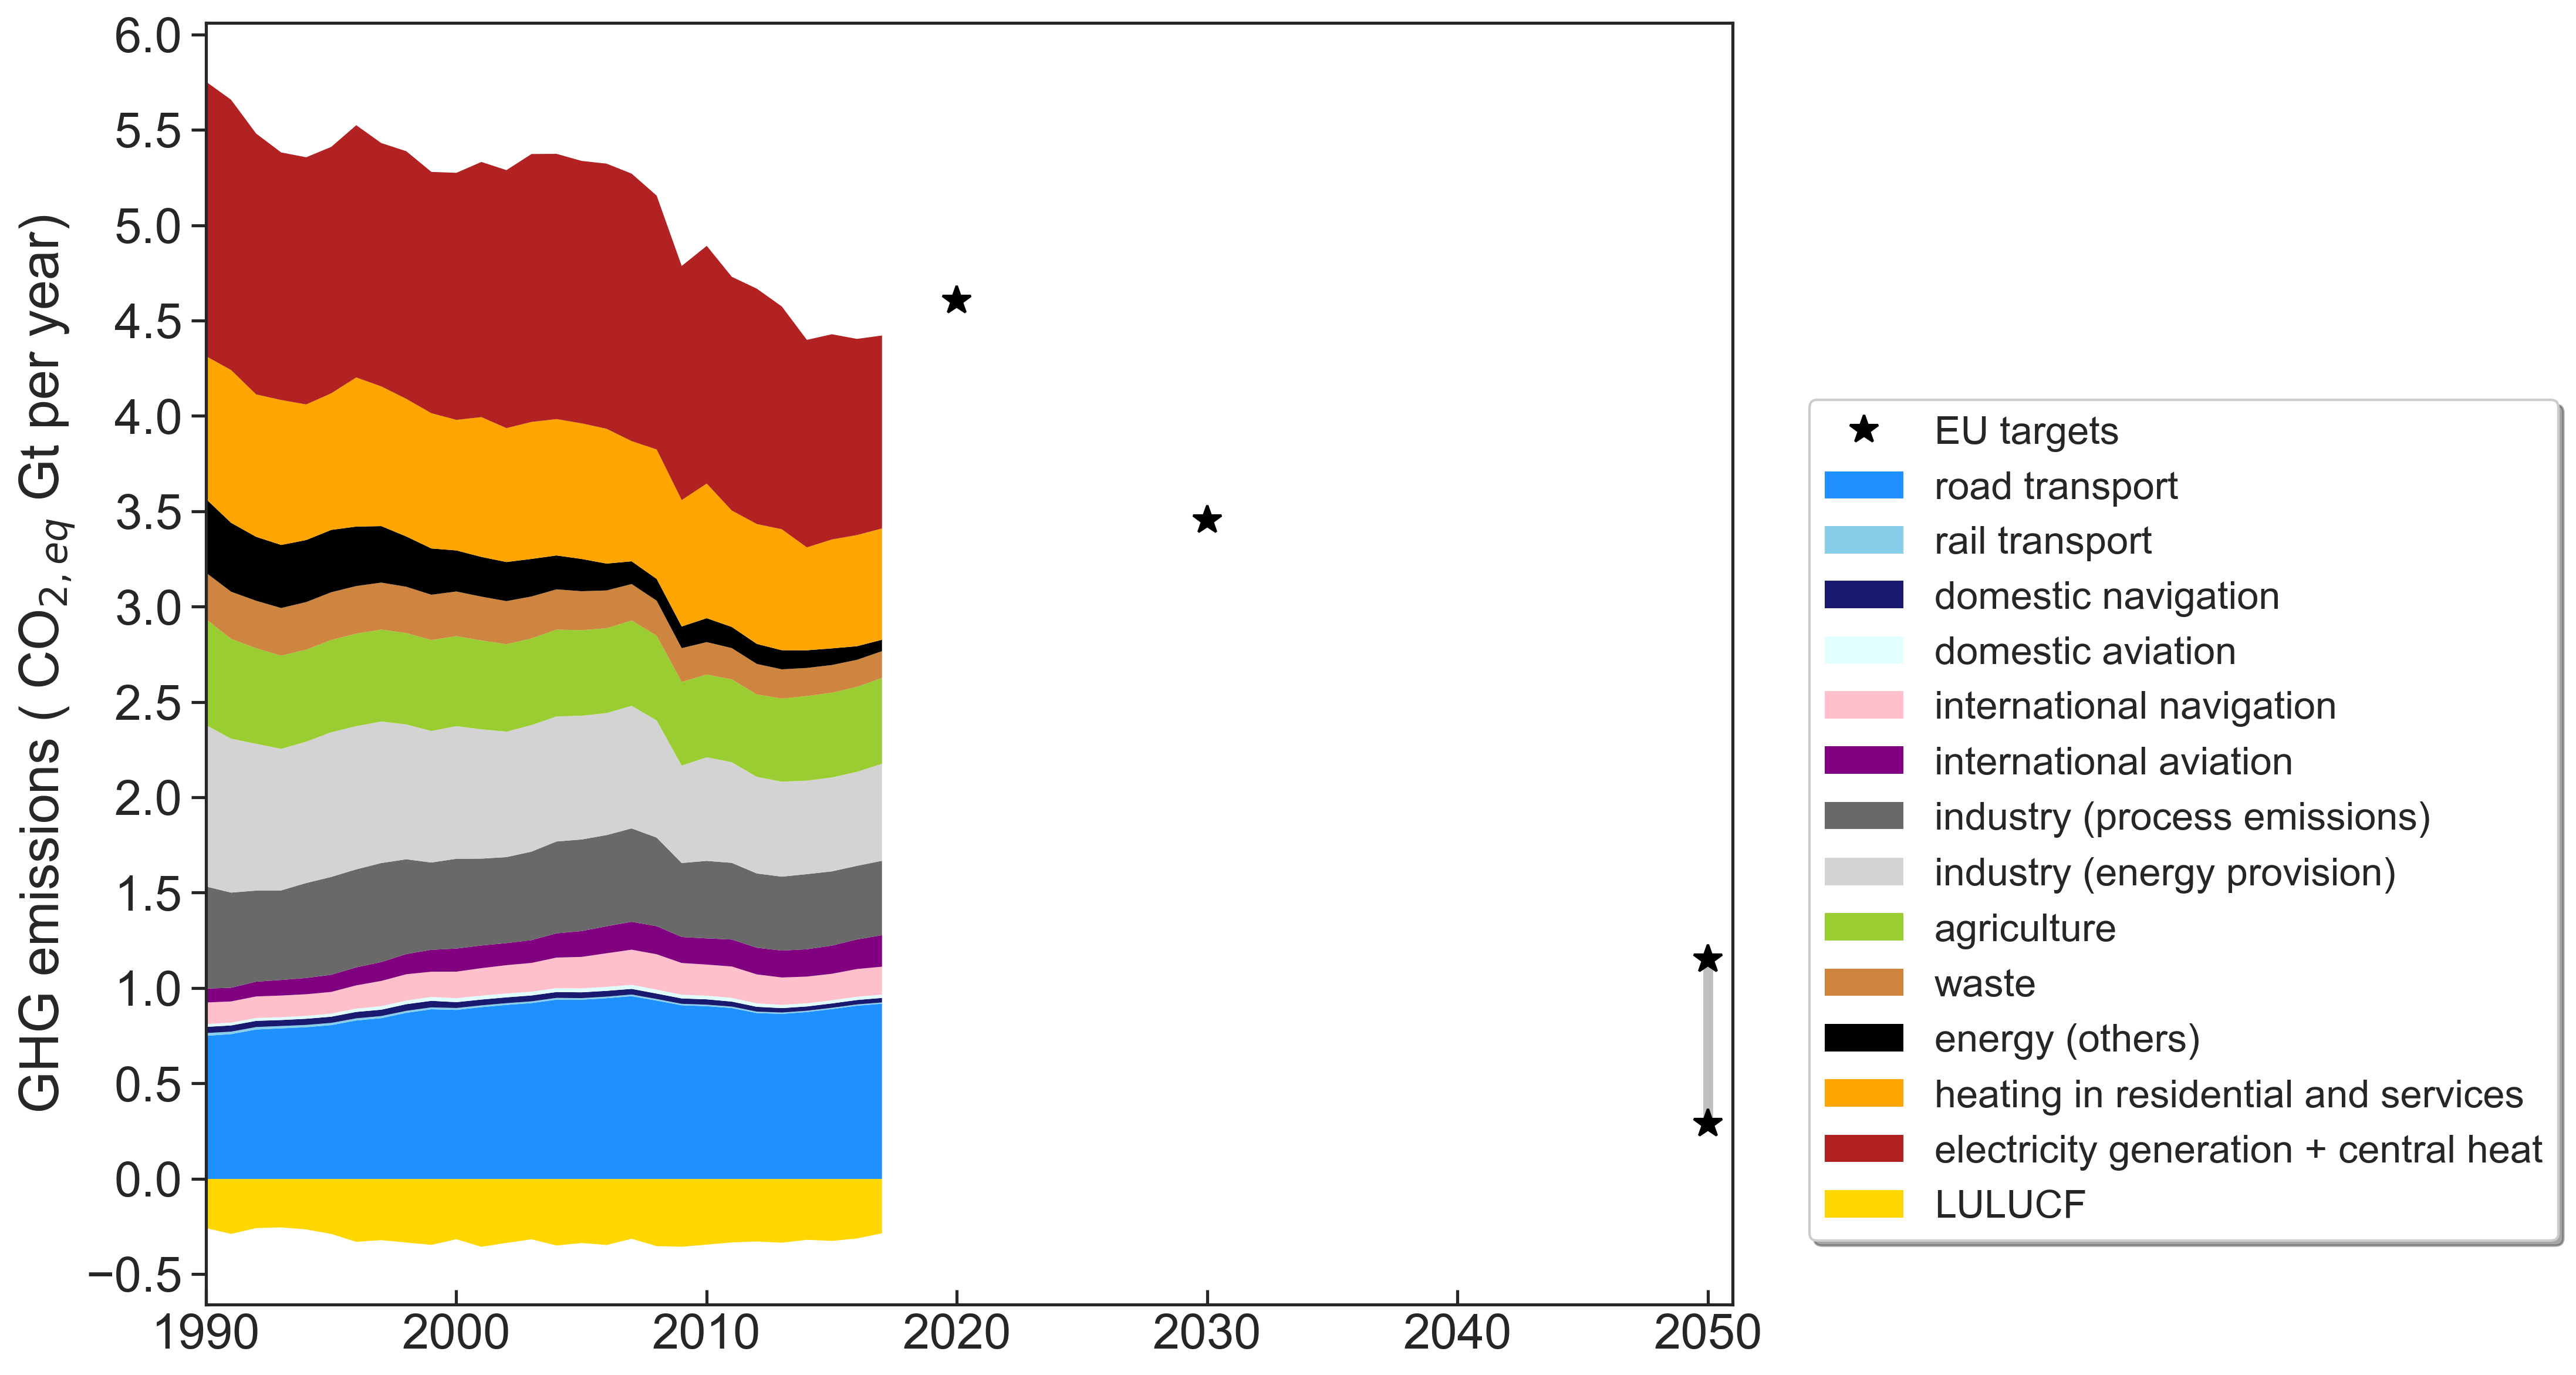
\includegraphics[width=\textwidth]{figures/historical_sectoral_emissions.png}
\caption{Sectoral distribution of historical emissions in the European Union \cite{UNFCCC_inventory}. The stars indicate committed EU reduction targets.} \label{fig_historical_emissions} 
\end{figure}

\section{CO$_2$ restriction paths with equivalent budget}

The $B$=21 GtCO$_2$ budget can be utilised following different transition paths. One option consists in assuming a linear CO$_2$ restriction path. Emissions will then reach zero in $t_f$

\begin{equation}
	t_f=t_0+\frac{2B}{e_0}
\end{equation}
where $t_0$=2020, and $e_0$ represents the carbon emissions from electricity and heating sector in 2020, which are assumed to be the same as in 2017. \\

Alternatively, emissions can be assumed to follow a path defined by one minus the cumulative distribution function (CDF$_\beta$) of a beta distribution in which $\beta_1$ = $\beta_2$. 

\begin{equation}
\begin{aligned}
&	e (t) = e_0(1- CDF_{\beta}(t)) \\
&	CDF_{\beta} (t) =\int_{-\infty}^{t} PDF_{\beta}(t) dt \\
&	PDF_{\beta} (t) =  \frac{\Gamma(\beta_1+\beta_2)}{\Gamma(\beta_1)+\Gamma(\beta_2)} t^{\beta_1-1} (1-t)^{\beta_2-1}
\end{aligned}
\end{equation}
where $\Gamma$ is the gamma function. The cumulative emissions fulfil $\int_{t_0}^{\infty} e(t) dt =B$. \\

The third option considered for the transition path is an exponential decay, following Raupach \textit{et al. }\cite{Raupach_2014}. In that case, emissions evolve as:
\begin{equation}
e(t) = e_0(1+(r+m)t)e^{-mt}
\end{equation}

where $r$ is the initial linear growth rate, which here is assumed to be $r$=0, and the decay parameter $m$ is determined by imposing the integral of the path to be equal to the budget.
\begin{equation}
\begin{aligned}
& B=\int_{t_0}^{\infty} e_0(1+(r+m)t)e^{-mt} dt \\
& m=\frac{1+ \sqrt{1+\frac{rB}{e_0}}}{\frac{B}{e_0}}
\end{aligned}
\end{equation}

Although the exponential decay path approaches asymptotically to zero, we assume here that $e(2050)=0$. By doing that, the final point of the different transition paths is equivalent and all of them achieve net-zero emissions by 2050.

\section{Historical evolution of CO$_2$ emissions from heating supply in residential and services sector in European countries}

\begin{figure}[!h]
\centering
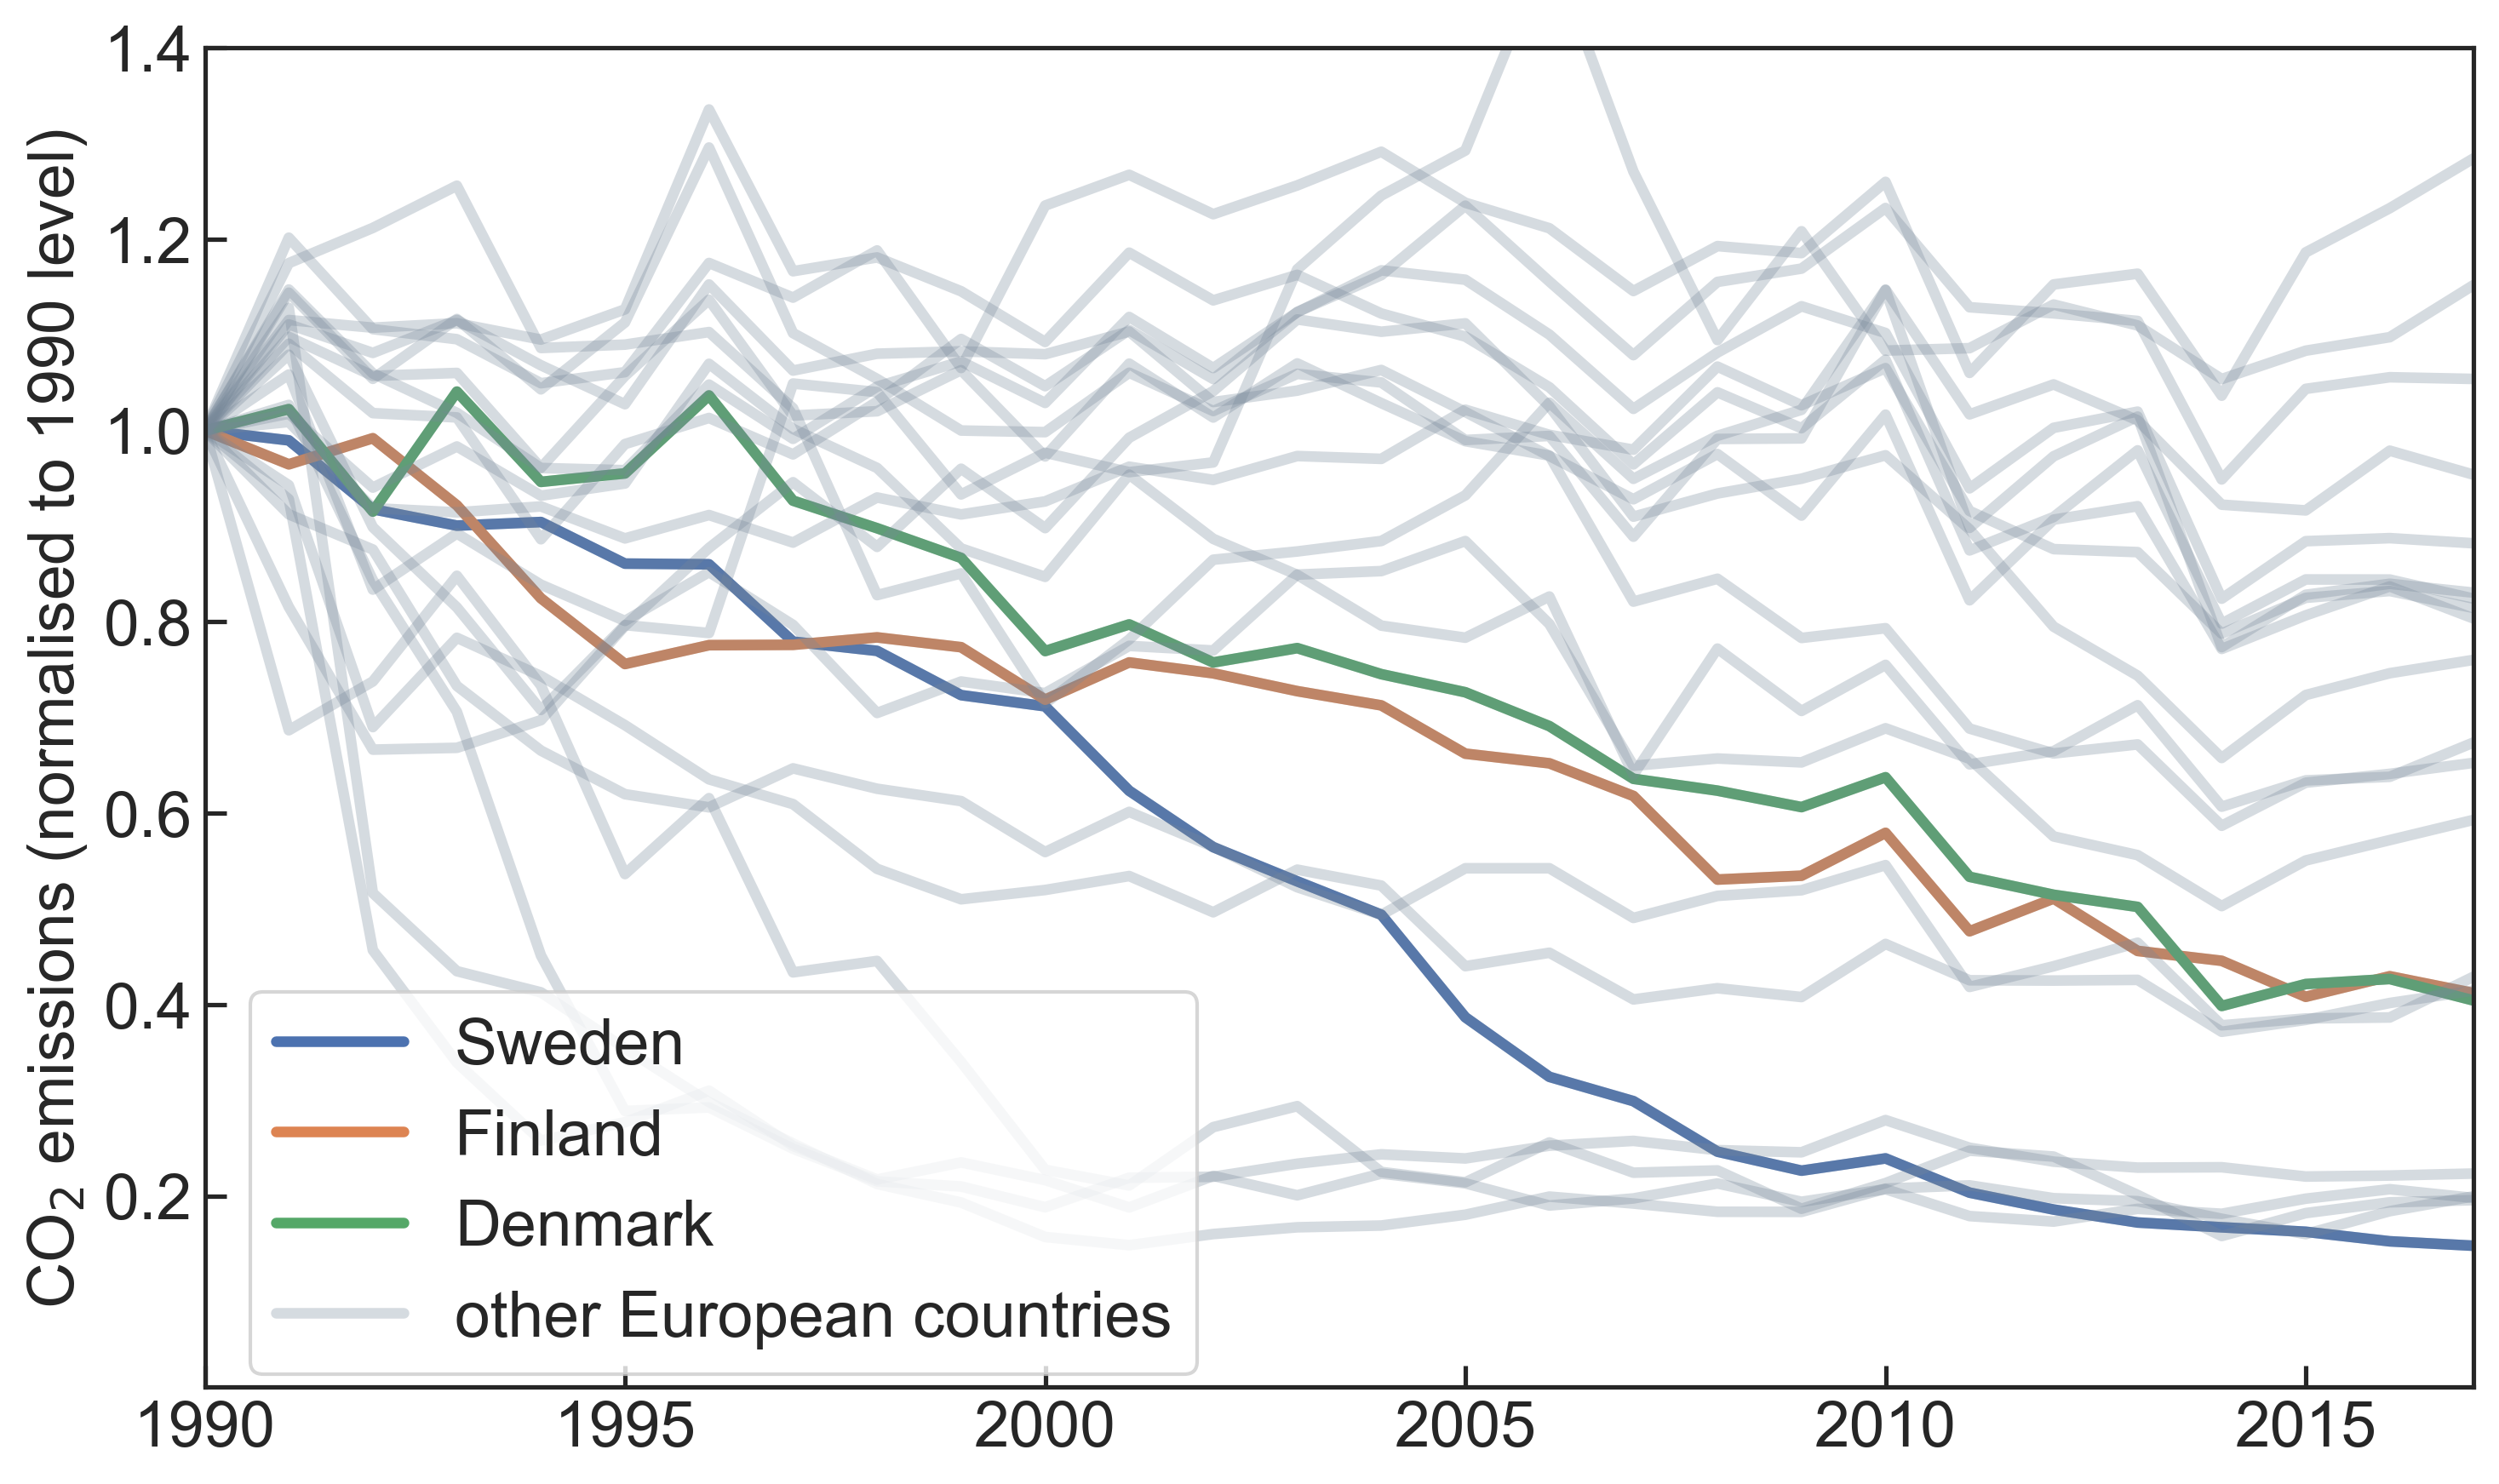
\includegraphics[width=12cm]{figures/emissions_heating.png}
\caption{Historical CO$_2$ emissions from heating in residential and services sector \cite{UNFCCC_inventory}. } \label{fig_emissions_heating} 
\end{figure}

\begin{figure}[!h]
\centering
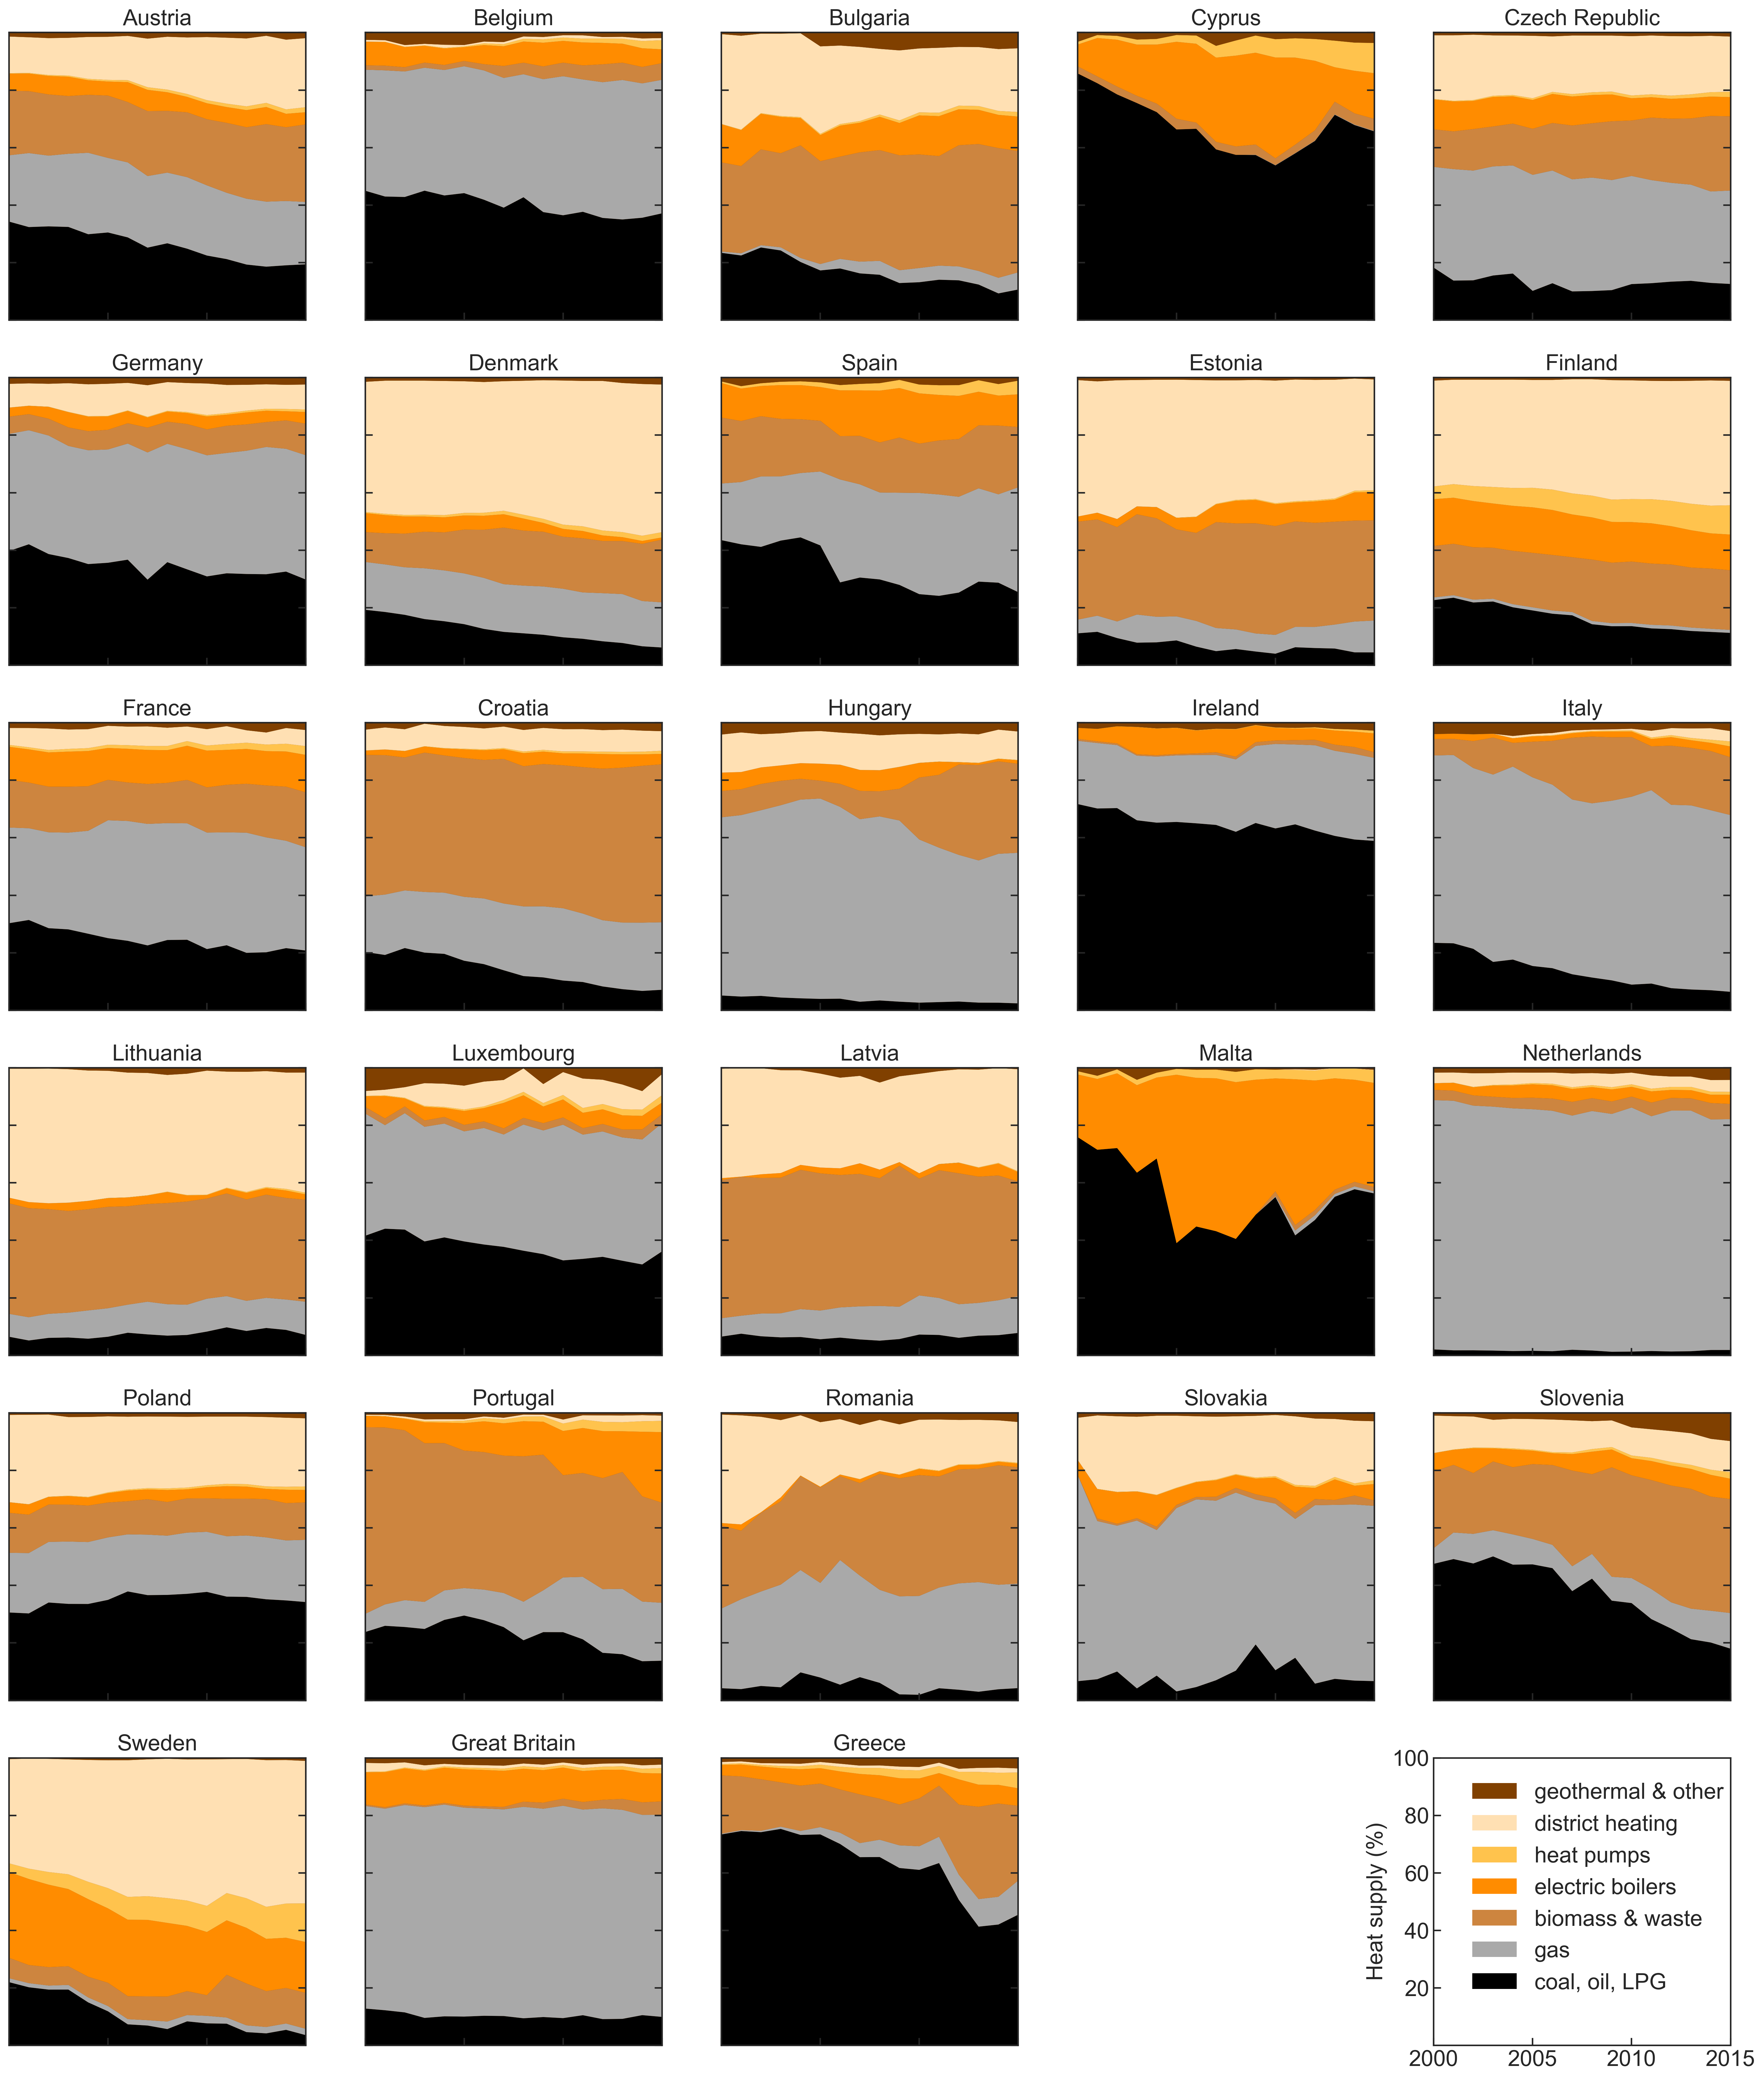
\includegraphics[width=\textwidth]{figures/heating_historical.png}
\caption{Historical share of technologies used to supply heating demand in residential and services sector \cite{IDEES}. } \label{fig_historical_heating} 
\end{figure}

\section{Power plants in operation in Europe}

\begin{figure}[!h]
\centering
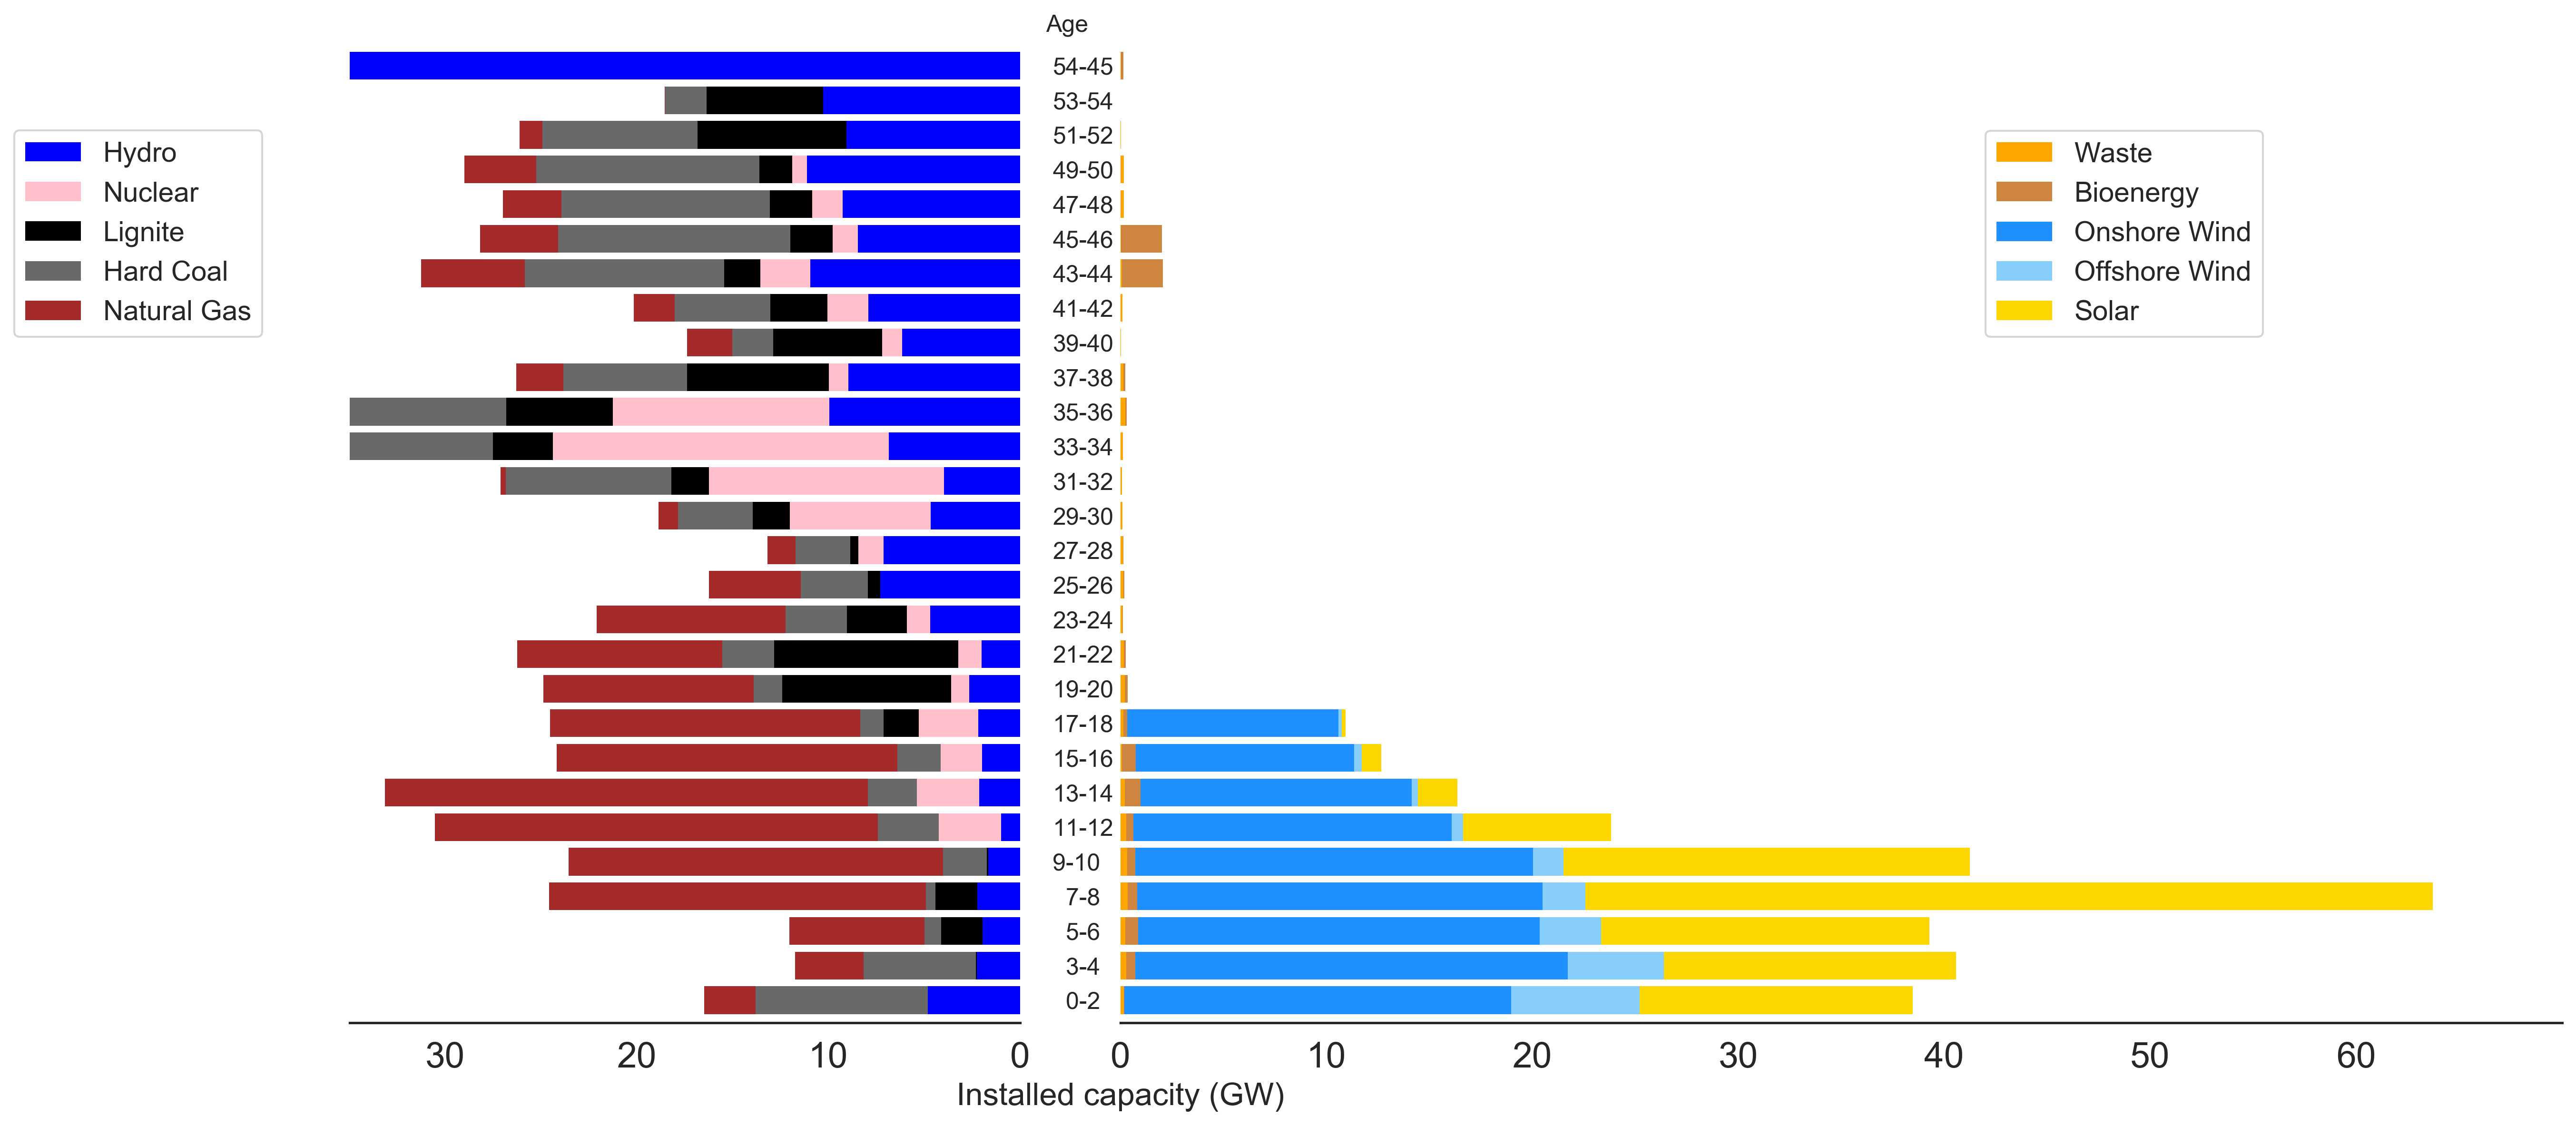
\includegraphics[width=\textwidth]{figures/age_distribution_2years_width.png}
\caption{Age distribution of European power plants in operation \cite{powerplantmatching, IRENA_2019}} \label{fig_age_distribution} 
\end{figure}

\section{Historical build rates for solar photovoltaics in European countries}

\begin{figure}[!h]
\centering
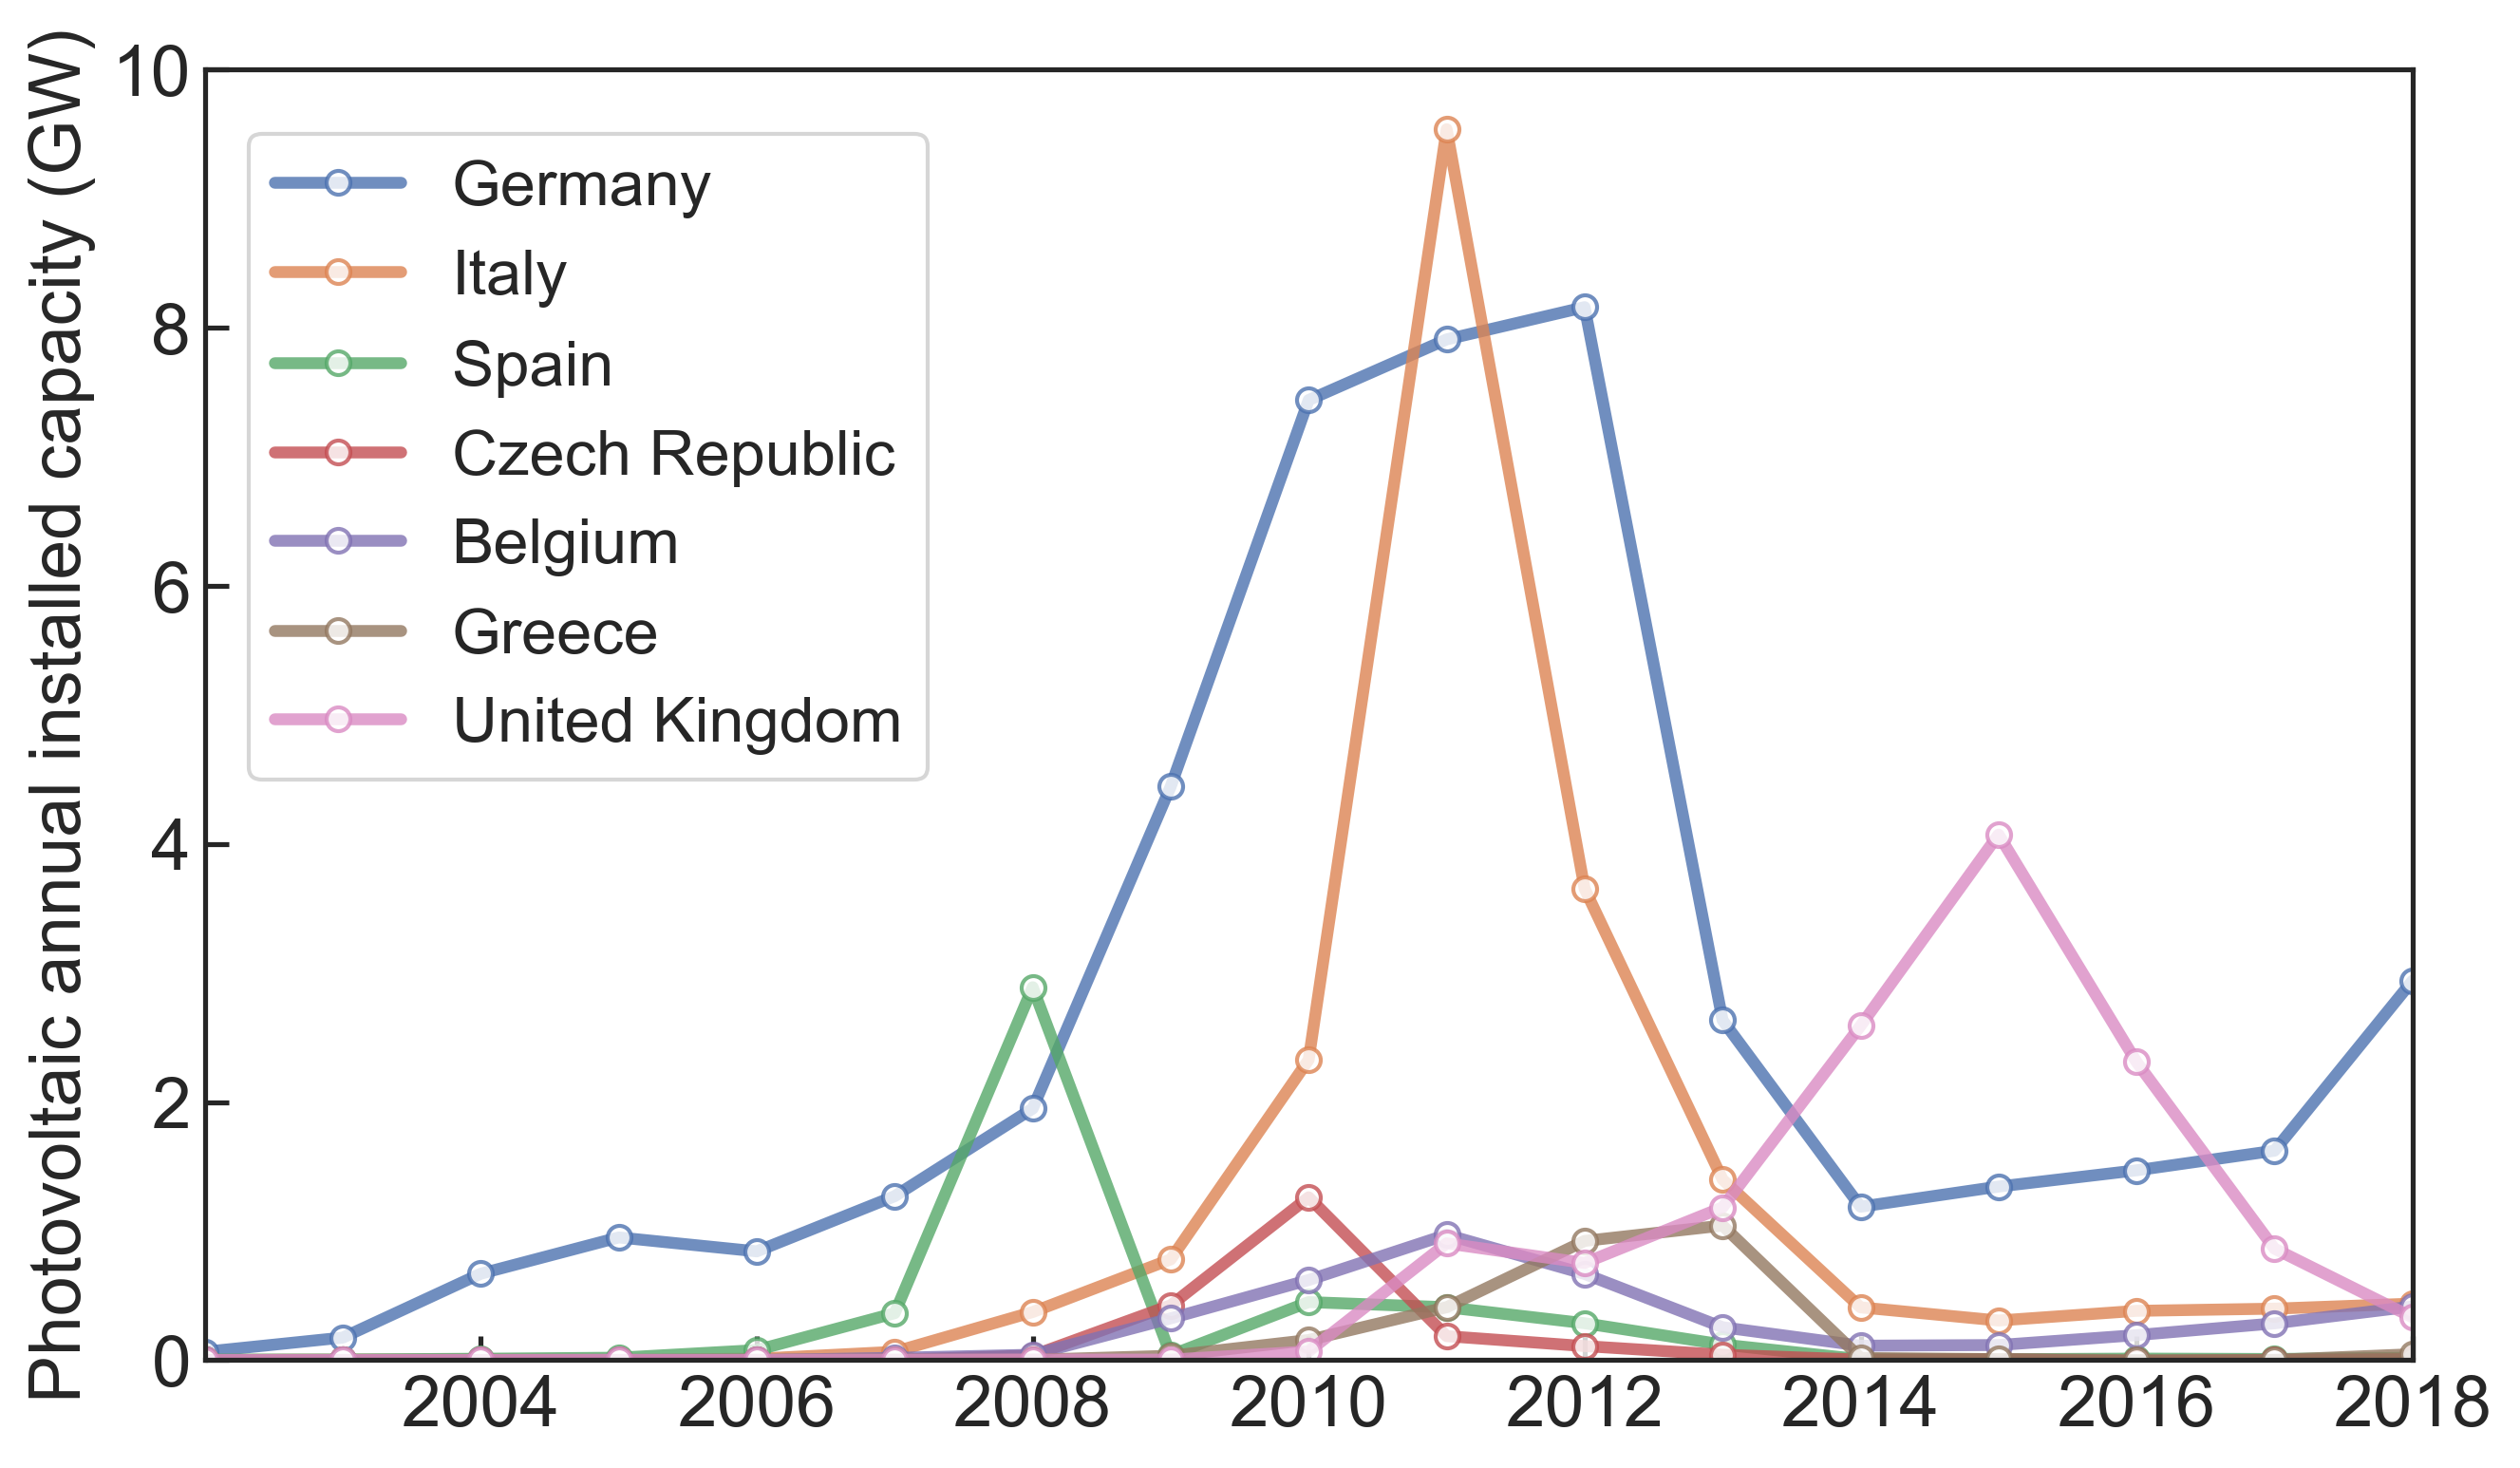
\includegraphics[width=12cm]{figures/installation_rates_PV.png}
\caption{Photovoltaic annual build rates for those European countries with a prominent peak \cite{IRENA_2019}. The sharp increase and subsequent decrease in the installation rates were caused by country-specific successive changes in the regulatory frameworks. See for instance \cite{Report_Fraunhofer_2019, Victoria_2012}. } \label{fig_installation_rates_PV} 
\end{figure}
 


\section{Transition paths cautious and last-minute. Additional results}

\begin{figure}[!h]
	\centering
	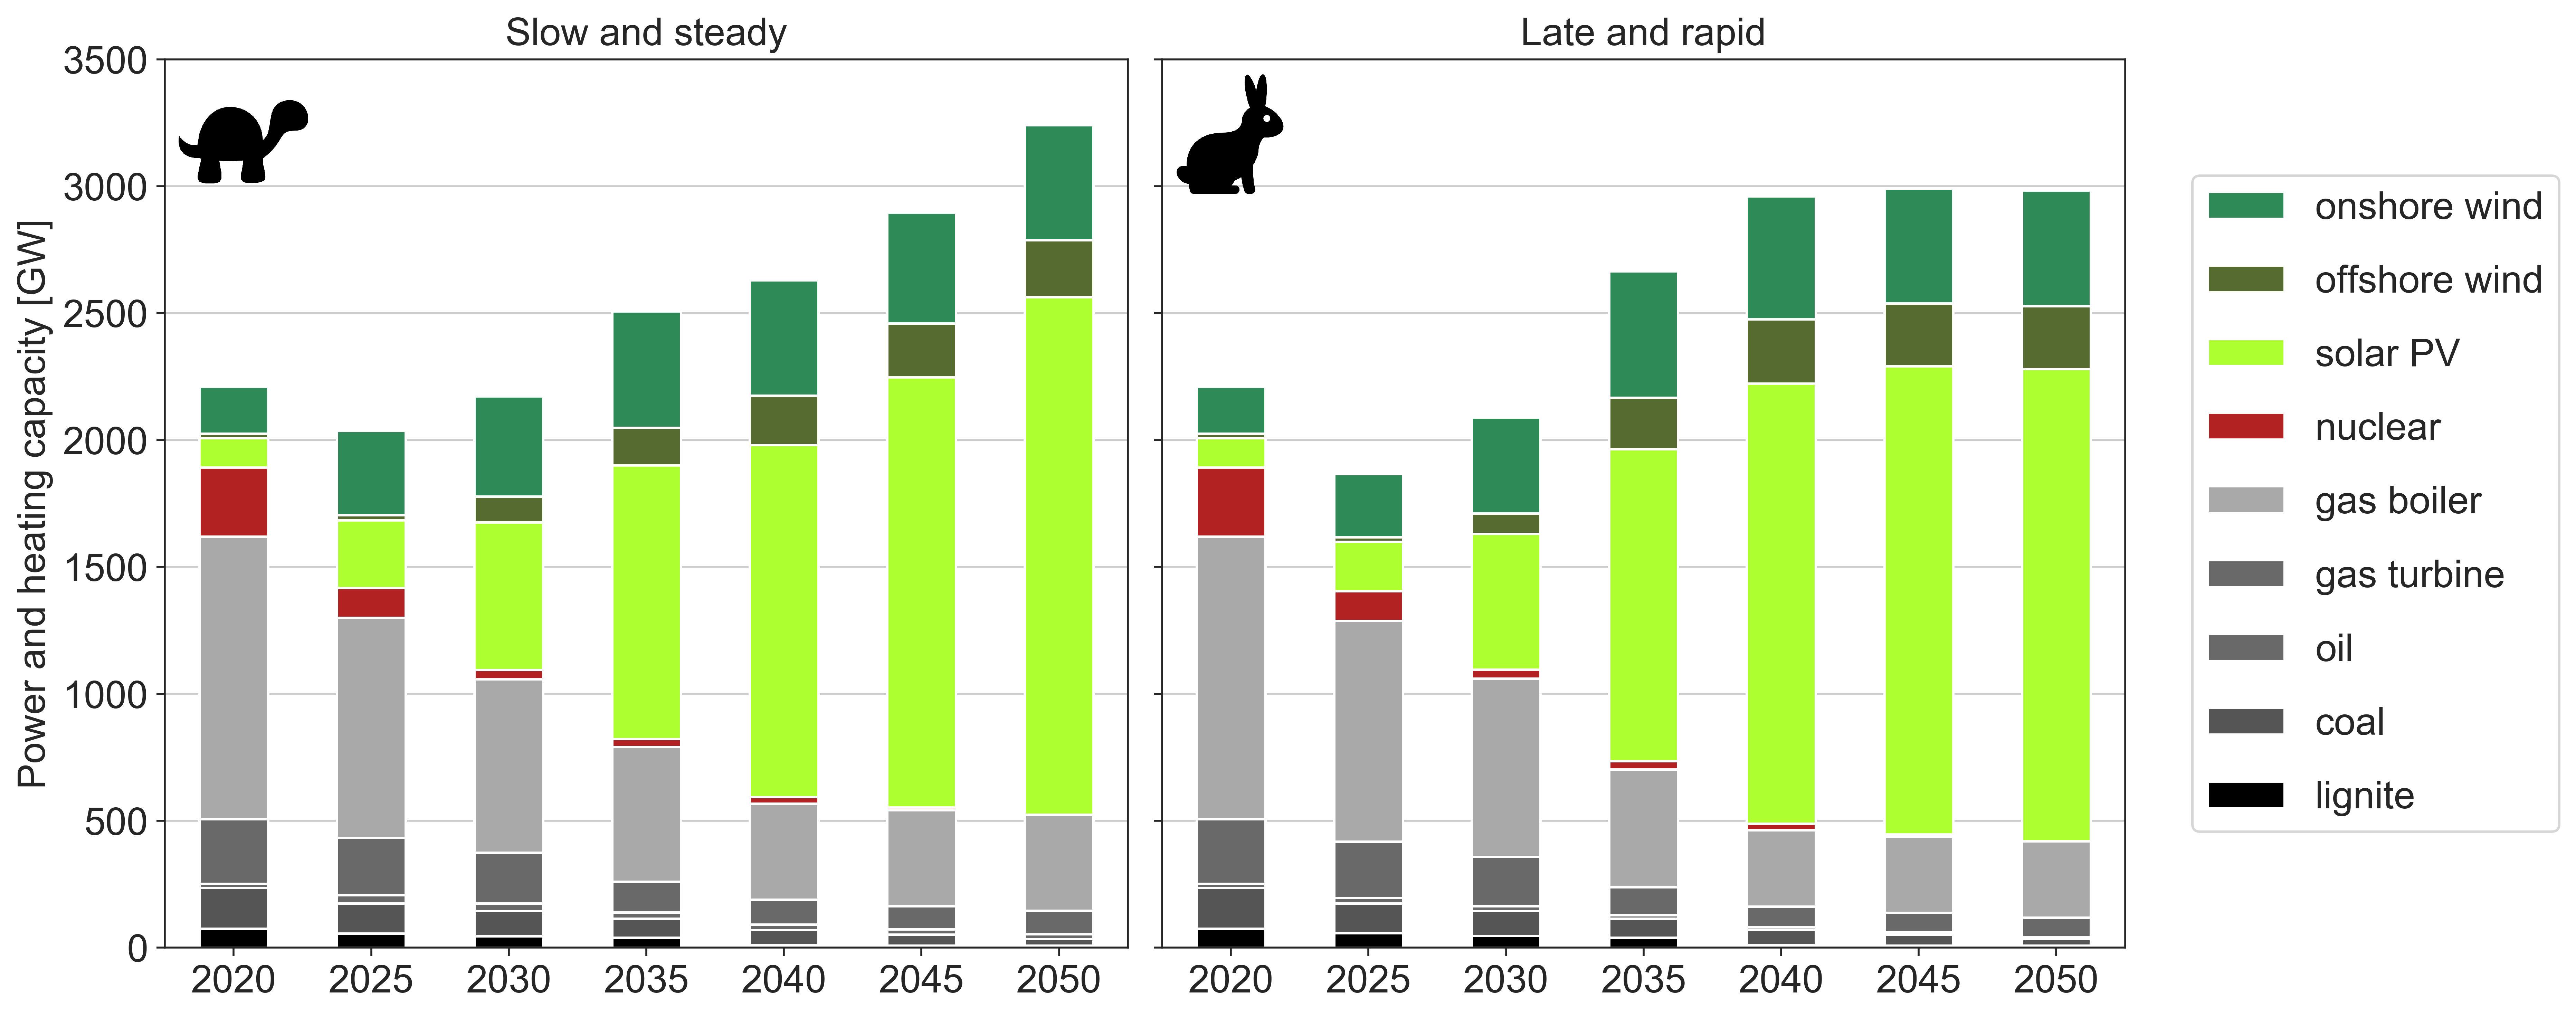
\includegraphics[width=12cm]{figures/installed_capacity_Base.png}
	\caption{Installed capacities for different technologies throughout transition paths cautious and last-minute shown in Fig. 1 in the main text.} \label{fig_installed_capacity} 
\end{figure}

\begin{figure}[!h]
\centering
%	\includegraphics[width=\columnwidth]{figures/spatial_plot_primary_energy.png}
\caption{Primary energy in every country in 2050. (left) Cautious transition path, (right) Greenfield optimization for 2050.} \label{fig_spatial_plot} 
\end{figure}

\begin{figure}[!h]
\centering
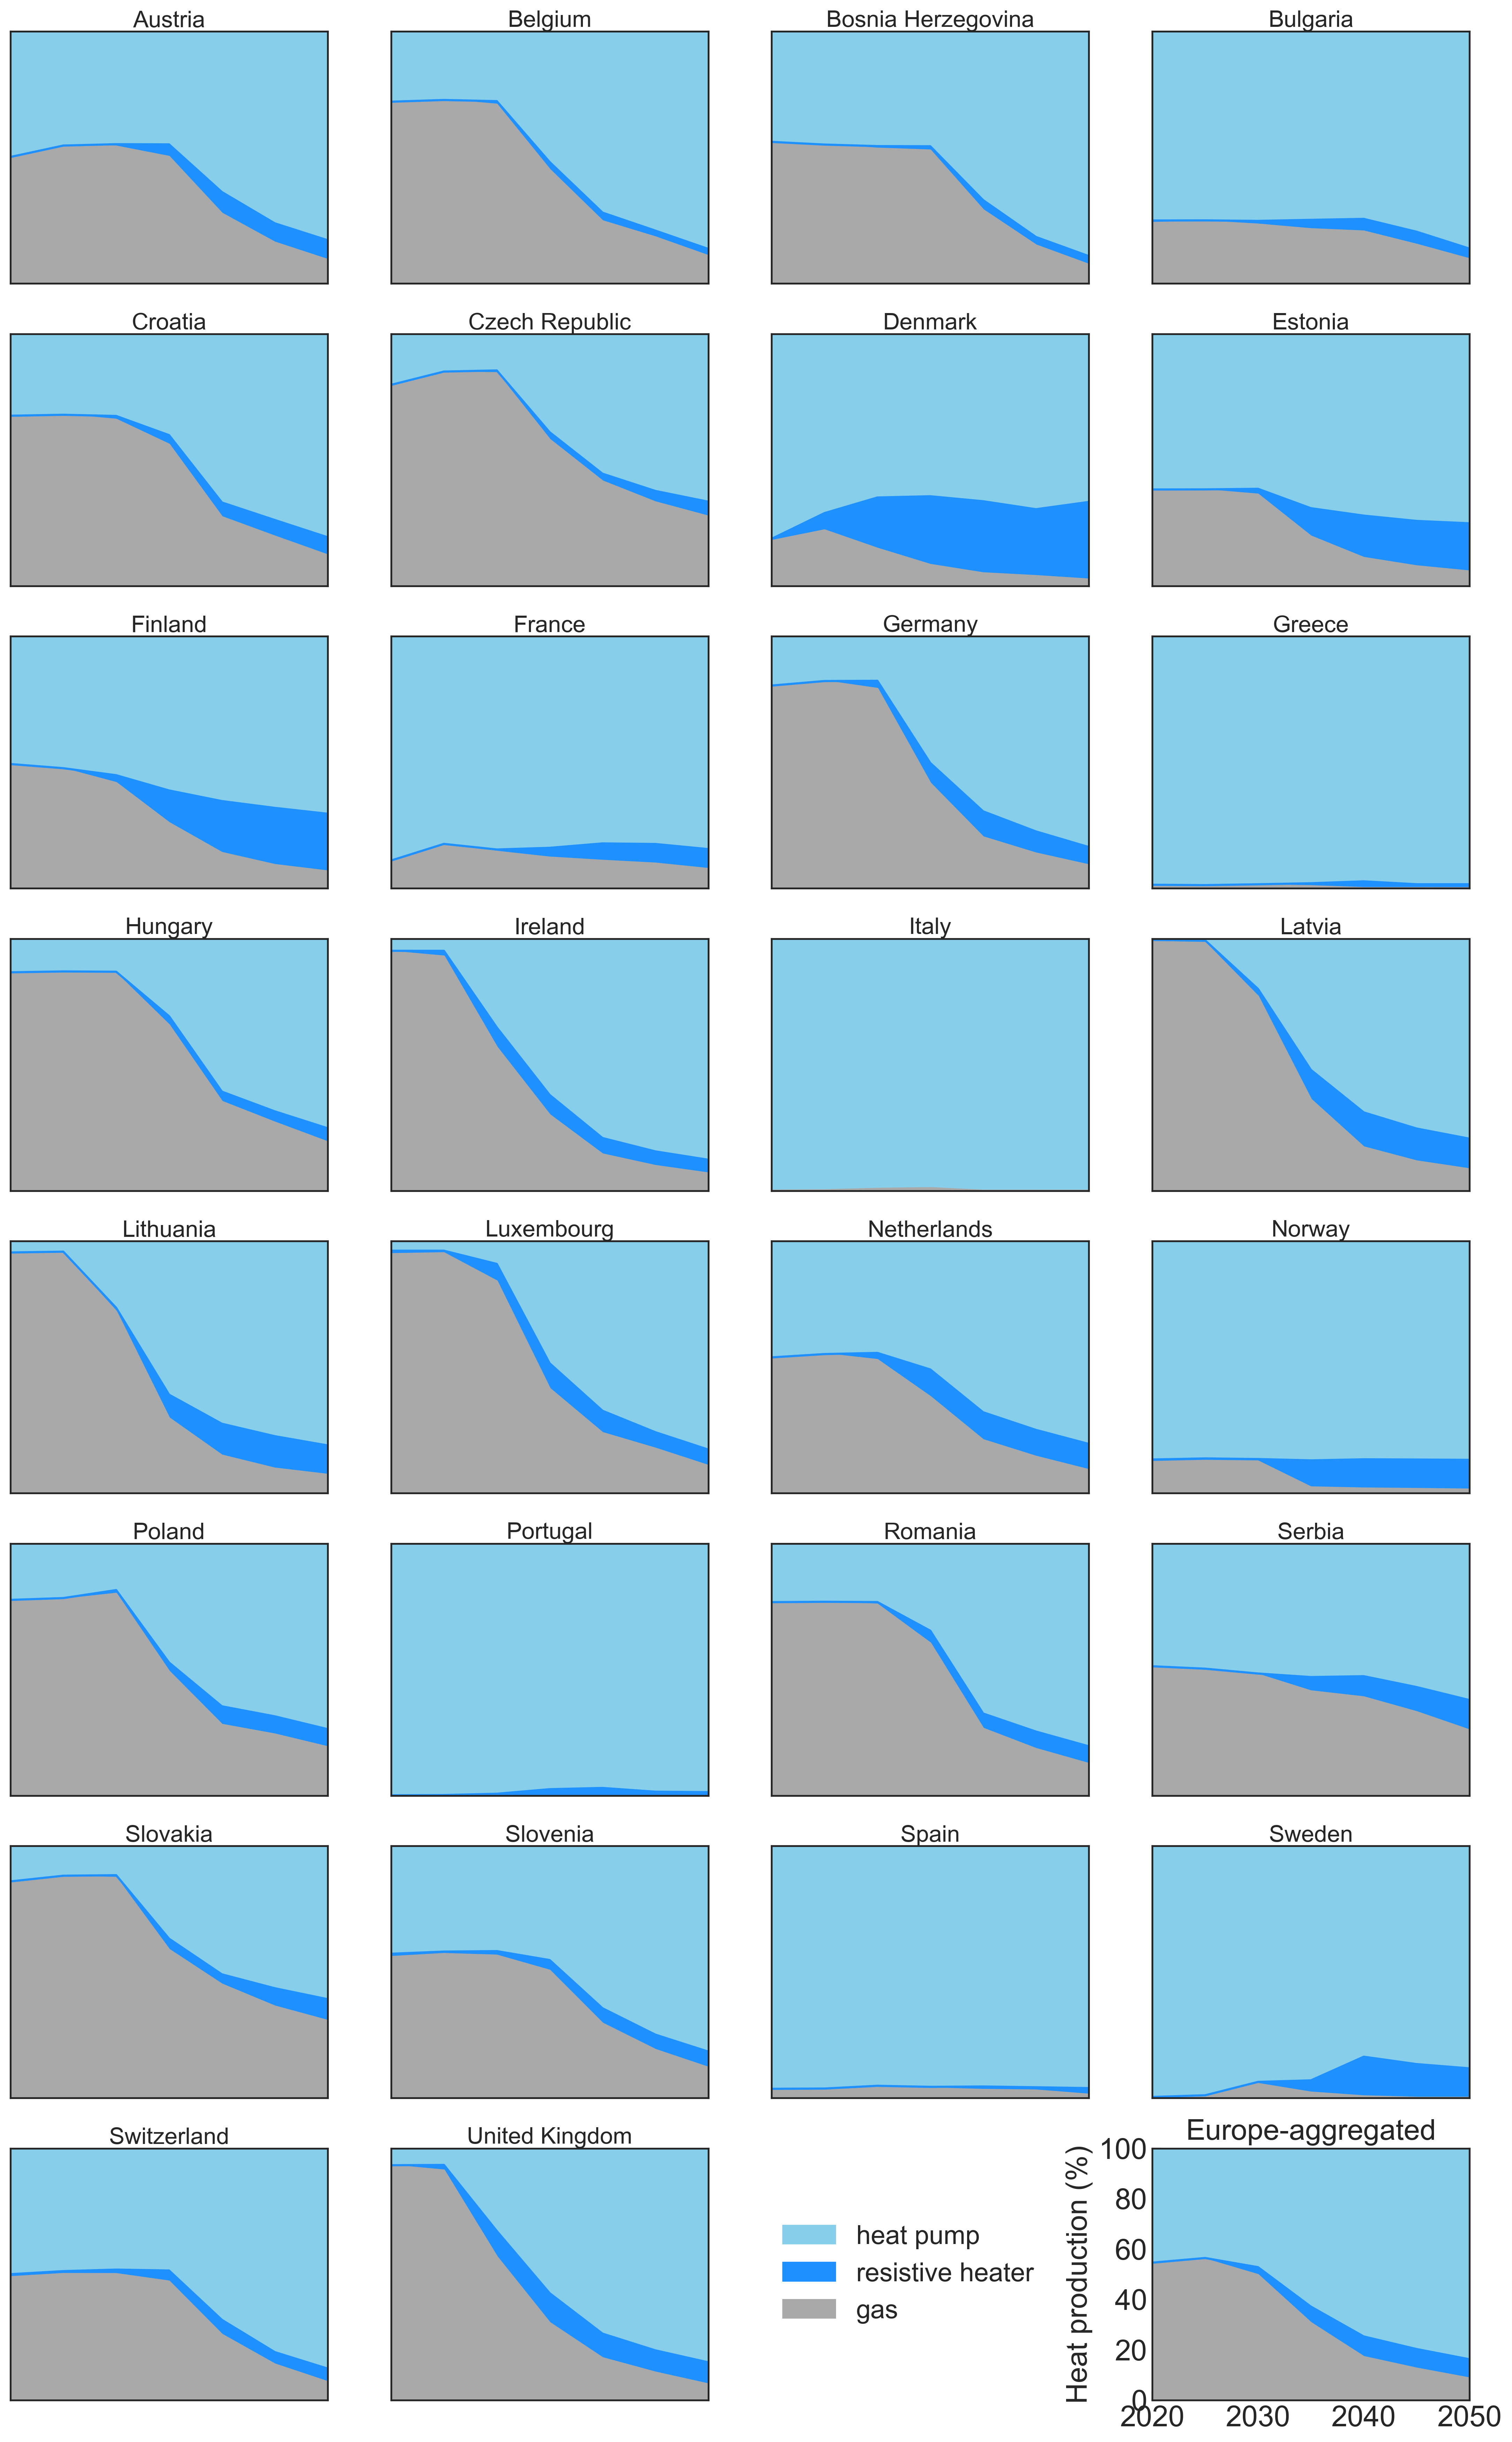
\includegraphics[width=14cm]{figures/heat_production_Base_go.png}
\caption{Evolution of technologies used to supply heating in residential and services sector in the cautious path. } \label{fig_heating_shares} 
\end{figure}

\FloatBarrier

\section{Model description}

In every time step, the optimisation objective, that is, the total annualised system cost is calculated as:

\begin{align}
& \min_{\substack{G_{n,s},E_{n,s},\\F_\ell,g_{n,s,t}}} \left[ \sum_{n,s} c_{n,s} \cdot G_{n,s} +\sum_{n,s} \hat{c}_{n,s} \cdot E_{n,s} \right. \nonumber \\
& \hspace{2cm} \left. + \sum_{\ell} c_{\ell} \cdot F_{\ell}+ \sum_{n,s,t} o_{n,s,t} \cdot g_{n,s,t} \right]
\label{eq_objective}
\end{align}

where $c_{n,s}$ are the fixed annualised costs for generator and storage power capacity $G_{n,s}$ of technology $s$ in every bus $n$, $\hat{c}_{n,s}$ are the fixed annualised costs for storage energy capacity $E_{n,s}$, $c_\ell$ are the fixed annualised costs for bus connectors $F_{\ell}$, and $o_{n,s,t}$ are the variable costs (which in some cases include CO$_2$ tax), for generation and storage dispatch $g_{n,s,t}$ in every hour $t$. Bus connectors $\ell$ include transmission lines but also converters between the buses implemented in every country (see Figure \ref{Fig_buses}), for instance, heat pumps that connect the electricity and heating bus. \\

The optimisation of the system is subject to several constraints. First, hourly demand $d_{n,t}$ in every bus $n$ must be supplied by generators in that bus or imported from other buses. $f_{\ell,t}$ represents the energy flow on the link $l$ and $\alpha_{n,\ell,t}$ indicates both the direction and the efficiency of flow on the bus connectors.  $\alpha_{n,\ell,t}$ can be time dependent such as in the case of heat pumps whose conversion efficiency depends on the ambient temperature.

\begin{equation}
\sum_{s} g_{n,s,t}+ \sum_{\ell} \alpha_{n,\ell,t}\cdot f_{\ell,t} = d_{n,t} \hspace{.2cm} \leftrightarrow \hspace{0.2cm} \lambda_{n,t} \hspace{.3cm} \forall\, n,t \label{eq_energy_balance}
\end{equation}

The Lagrange multiplier $\lambda_{n,t}$,  also known as Karun-Kush-Tucker (KKT),  associated with the demand constraint indicates the marginal price of the energy carrier in the bus $n$, \textit{e.g.}, local marginal electricity price in the electricity bus. \\

Second, the maximum power flowing through the links is limited by their maximum physical capacity $F_{\ell}$. For transmission links, $\ubar{f}_{\ell,t}=-1$ and $\bar{f}_{\ell,t}=1$, which allows both import and export between neighbouring countries. For a unidirectional converter \textit{e.g.}, a heat resistor, $\ubar{f}_{\ell,t}=0$ and $\bar{f}_{\ell,t}=1$ since a heat resistor can only convert electricity into heat.

\begin{equation}
\ubar{f}_{\ell,t} \cdot F_{\ell} \leq f_{\ell,t} \leq \bar{f}_{\ell,t} \cdot F_{\ell} \hspace{1cm} \forall\, \ell,t \; . \label{eq_links}
\end{equation}

For interconnecting transmission lines, the lengths $l_{\ell}$ are set by the distance between the geographical mid-points of each country, so that some of the transmission within each country is also reflected in the optimisation. A factor of 25\% is added to the line lengths to account for the fact that transmission lines cannot be placed as the crow flies due to land use restriction. For the transmission lines capacities $F_{\ell}$, a safety margin of 33\% of the installed capacity is used to satisfy n-1 requirements \cite{Brown_2016}. \\ %Linear optimal power flow is applied using Kirchhoff's formulation \cite{Horsch_2018}. 

Third, for every hour the maximum capacity that can provide a generator or storage is bounded by the product between installed capacity $G_{n,s}$ and availabilities $\ubar{g}_{n,s,t}$, $\bar{g}_{n,s,t}$. For instance, for solar generators $\ubar{g}_{n,s,t}$ is zero and $\bar{g}_{n,s,t}$ refers to the capacity factor at time $t$ 

\begin{equation}
\ubar{g}_{n,s,t} \cdot G_{n,s} \leq g_{n,s,t} \leq \bar{g}_{n,s,t} \cdot G_{n,s} \hspace{1cm} \forall\, n,s,t \; . \label{eq_g}
\end{equation}

The maximum power capacity for generators is limited by potentials $\bar{G}_{n,s}$ that are estimated taking into account physical and environmental constraints:
\begin{equation}\label{eq_max_G}
0 \leq G_{n,s}\leq \bar{G}_{n,s} \hspace{1cm} \forall\, n,s \; .
\end{equation}

The storage technologies have a charging efficiency $\eta_{in}$ and rate $g_{n,s,t}^+$, a discharging efficiency $\eta_{out}$ and rate $g_{n,s,t}^-$, possible inflow $g_{n,s,t,\textrm{inflow}}$ and spillage $g_{n,s,t,\textrm{spillage}}$, and standing loss $\eta_0$. The state of charge $e_{n,s,t}$ of every storage has to be consistent with charging and discharging in every hour and is limited by the energy capacity of the storage $E_{n,s}$. It should be remarked that the storage energy capacity $E_{n,s}$ can be optimised independently of the storage power capacity $G_{n,s}$.

\begin{align}
e_{n,s,t} = & \ \eta_0 \cdot e_{n,s,t-1} + \eta_{in} |g_{n,s,t}^+| - \eta_{out}^{-1} |g_{n,s,t}^-| \nonumber \\
& + g_{n,s,t,\textrm{inflow}} - g_{n,s,t,\textrm{spillage}} \; , \nonumber \\
& 0  \leq   e_{n,s,t} \leq E_{n,s}   \hspace{0.5cm} \forall\, n,s,t \; . \label{eq_storage}
\end{align}

So far, equations (\ref{eq_energy_balance}) to (\ref{eq_storage}) represent mainly technical constraints but additional constraints can be imposed to bound the solution.\\

The interconnecting transmission expansion can be limited by a global constraint
\begin{equation}
\sum_{\ell} l_\ell \cdot F_{\ell} \leq  \textrm{CAP}_{LV} \hspace{.7cm} \leftrightarrow \hspace{0.3cm} \mu_{LV} \; ,
%\hspace{.3cm} 
\label{eq_cap}
\end{equation}
where the sum of transmission capacities $F_{\ell}$ multiplied by the lengths $l_{\ell}$ is bounded by a transmission volume cap $\textrm{CAP}_{LV}$. In this case, the Lagrange/KKT multiplier $\mu_{LV}$ represents the shadow price of a marginal increase in transmission volume.\\


The maximum CO$_2$ allowed to be emitted by the system $\textrm{CAP}_{CO2}$ can be imposed through the constraint 

\begin{equation}
  \sum_{n,s,t}  \varepsilon_{s} \frac{ g_{n,s,t} }{\eta_{n,s}} + \sum_{n,s} \varepsilon_{s} (e_{n,s,t=0} - e_{n,s,t=T})  \leq  \textrm{CAP}_{CO2} \hspace{.4cm} \leftrightarrow \hspace{0.3cm} \mu_{CO2} \label{eq_co2cap}
\end{equation}

where $\varepsilon_{s}$ represents the specific emissions in CO$_2$-tonne-per-MWh\th{} of the fuel $s$, $\eta_{n,s}$ the efficiency and $g_{n,s,t}$ the generators dispatch. In this case, the Lagrange/KKT multiplier represents the shadow price of CO$_2$, \textit{i.e.}, the additional price that should be added for every unit of CO$_2$ to achieve the CO$_2$ reduction target in an open market. 

\section{Sectors description and data}

\textcolor[rgb]{1,0,0}{TODO: Add figure with the sectors included.}

\subsection{Electricity sector}
Hourly electricity demand for every country corresponding to 2015 is retrieved from EU Network Transmission System Operators of Electricity (ENTSO-E) via the convenient dataset prepared by the Open Power System Data (OPSD) initiative \cite{OPSD}. In every country, electricity can be generated by solar PV, onshore wind, offshore wind, Open Cycle Gas Turbines (OCGT), Combined Cycle Gas Turbines (CCGT), coal, lignite, and nuclear power plants and CHP units, with the costs, lifetimes and efficiencies shown in Table \ref{tab:cost per year}. Time series representing the hourly capacity factors for solar PV were obtained by converting weather data into solar electricity generation, assuming a uniform capacity layout across every country. Details on the conversion and aggregation methodology can be found in \cite{Victoria_2019b}, the complete time series dataset is available in \href{https://doi.org/10.5281/zenodo.1321809}{10.5281/zenodo.1321809}. CHP units are modelled as extraction condensing units, the feasible space representing the possible combinations of power and heat outputs is included as a constraint in the model, as detailed in \cite{Brown_2018}. \

\textcolor[rgb]{1,0,0}{TODO: Describe onshore/offshore time series.}

\textcolor[rgb]{1,0,0}{TODO: Describe maximum capacities. }

The transmission links between countries are assumed to be high-voltage direct current (HVDC) connections. For 2020 and 2030, the capacities correspond to the values assumed in the ENTSOE Ten-Year Network Development Plan (TNYDP), see Table \ref{tab_interconnections} and \cite{TYNDP2016}. The values for 2025 are interpolated assuming a liner capacity expansion between 2020 and 2030 for every link. For years from 2035 onwards, capacities are optimized together with the rest of the system components using 2030 values as the lower boundary. \textcolor[rgb]{1,0,0}{TODO: Describe other scenarios} \

\begin{table*}
\centering
\caption{Transmission capacities (MW) for interconnections \cite{TYNDP2016}.} \label{tab_interconnections}
\begin{tabular}{|lrr|lrr|lrr|}
\hline
Link & 2020 & 2030 & Link & 2020 & 2030 & Link & 2020 & 2030  \\
\hline
 AL-GR & 250 & 250 & FI-EE & 1000 & 1000 & LU-FR & 0 & 0 \\ AL-ME & 350 & 350 & FI-NO & 0 & 0 & LV-EE & 1600 & 1600 \\ AL-MK & 200 & 200 & FI-SE & 2300 & 2800 & LV-LT & 1200 & 1800 \\ AL-RS & 760 & 760 & FR-BE & 4300 & 4300 & ME-AL & 350 & 350 \\ AT-CH & 1700 & 1700 & FR-CH & 3700 & 3700 & ME-BA & 400 & 400 \\ AT-CZ & 1000 & 1000 & FR-DE & 3000 & 4800 & ME-IT & 1200 & 1200 \\ AT-DE & 5000 & 7500 & FR-ES & 5000 & 8000 & ME-RS & 1000 & 1000 \\ AT-HU & 1200 & 1200 & FR-GB & 5400 & 5400 & MK-AL & 200 & 200 \\ AT-IT & 555 & 1655 & FR-IE & 0 & 700 & MK-BG & 150 & 150 \\ AT-SI & 1200 & 1200 & FR-IT & 4350 & 4350 & MK-GR & 400 & 400 \\ BA-HR & 1344 & 1844 & FR-LU & 380 & 380 & MK-RS & 1050 & 1050 \\ BA-ME & 500 & 500 & GB-BE & 1000 & 1000 & NI-GB & 80 & 500 \\ BA-RS & 1100 & 1100 & GB-DK & 1400 & 1400 & NI-IE & 1100 & 1100 \\ BE-DE & 1000 & 1000 & GB-FR & 5400 & 5400 & NL-BE & 2400 & 2400 \\ BE-FR & 2800 & 2800 & GB-IE & 500 & 500 & NL-DE & 4450 & 5000 \\ BE-GB & 1000 & 1000 & GB-IS & 0 & 0 & NL-DK & 700 & 700 \\ BE-LU & 1080 & 1080 & GB-NI & 500 & 500 & NL-GB & 1000 & 1000 \\ BE-NL & 2400 & 2400 & GB-NL & 1000 & 1000 & NL-NO & 700 & 700 \\ BG-GR & 1728 & 1728 & GB-NO & 1400 & 1400 & NO-DE & 1400 & 1400 \\ BG-MK & 530 & 530 & GR-AL & 250 & 250 & NO-DK & 1640 & 1640 \\ BG-RO & 1400 & 1400 & GR-BG & 1032 & 1032 & NO-FI & 0 & 0 \\ BG-RS & 600 & 600 & GR-CY & 2000 & 2000 & NO-GB & 1400 & 1400 \\ CH-AT & 1700 & 1700 & GR-IT & 500 & 500 & NO-NL & 700 & 700 \\ CH-DE & 4700 & 4700 & GR-MK & 350 & 350 & NO-SE & 3695 & 3695 \\ CH-FR & 1300 & 1300 & HR-BA & 1312 & 1812 & PL-CZ & 600 & 600 \\ CH-IT & 6240 & 6240 & HR-HU & 2000 & 2000 & PL-DE & 3000 & 3000 \\ CY-GR & 2000 & 2000 & HR-IT & 0 & 0 & PL-DK & 0 & 0 \\ CZ-AT & 1200 & 1200 & HR-RS & 600 & 600 & PL-LT & 1000 & 1000 \\ CZ-DE & 2100 & 2600 & HR-SI & 2000 & 2000 & PL-PL & 5000 & 5000 \\ CZ-PL & 500 & 500 & HU-AT & 800 & 800 & PL-SE & 600 & 600 \\ CZ-SK & 2100 & 2100 & HU-HR & 2000 & 2000 & PL-SK & 990 & 990 \\ DE-AT & 5000 & 7500 & HU-RO & 1300 & 1300 & PT-ES & 3500 & 3500 \\ DE-BE & 1000 & 1000 & HU-RS & 600 & 600 & RO-BG & 1500 & 1500 \\ DE-CH & 3286 & 3286 & HU-SI & 1700 & 1700 & RO-HU & 1400 & 1400 \\ DE-CZ & 1500 & 2000 & HU-SK & 2000 & 2000 & RO-RS & 1450 & 1450 \\ DE-DK & 4000 & 4000 & IE-FR & 0 & 700 & RS-AL & 330 & 330 \\ DE-FR & 3000 & 4800 & IE-GB & 500 & 500 & RS-BA & 1200 & 1200 \\ DE-LU & 2300 & 2300 & IE-NI & 1100 & 1100 & RS-BG & 350 & 350 \\ DE-NL & 4450 & 5000 & IS-GB & 0 & 0 & RS-HR & 600 & 600 \\ DE-NO & 1400 & 1400 & IT-AT & 385 & 1385 & RS-HU & 600 & 600 \\ DE-PL & 2000 & 2000 & IT-CH & 3860 & 3860 & RS-ME & 1100 & 1100 \\ DE-SE & 615 & 1315 & IT-FR & 2160 & 2160 & RS-MK & 950 & 950 \\ DK-DE & 4000 & 4000 & IT-GR & 500 & 500 & RS-RO & 1050 & 1050 \\ DK-DK & 1200 & 1200 & IT-HR & 0 & 0 & SE-DE & 615 & 1315 \\ DK-GB & 1400 & 1400 & IT-IT & 5750 & 5750 & SE-DK & 1980 & 1980 \\ DK-NL & 700 & 700 & IT-ME & 1200 & 1200 & SE-FI & 2400 & 3200 \\ DK-NO & 1640 & 1640 & IT-SI & 1380 & 1380 & SE-LT & 700 & 700 \\ DK-PL & 0 & 0 & IT-TN & 0 & 0 & SE-NO & 3995 & 3995 \\ DK-SE & 2440 & 2440 & LT-LV & 1500 & 2100 & SE-PL & 600 & 600 \\ EE-FI & 1016 & 1016 & LT-PL & 1000 & 1000 & SI-AT & 1200 & 1200 \\ EE-LV & 1600 & 1600 & LT-SE & 700 & 700 & SI-HR & 2000 & 2000 \\ ES-FR & 5000 & 8000 & LU-BE & 700 & 700 & SI-HU & 2000 & 2000 \\ ES-PT & 4200 & 4200 & LU-DE & 2300 & 2300 & SI-IT & 1530 & 1530 \\
\hline
\end{tabular}
\end{table*}

\subsubsection{Existing power plants and decommissioning}

For conventional technologies, \textit{i.e.} OCGT, CCGT, coal, lignite, nuclear and CHP, installed capacities in every country in 2020 and commissioning dates are retrieved from \cite{powerplantmatching}. 
A two-step method was implemented to fill commissioning date for power plants whose data was missing. First, for units larger than 50 MW, commissioning dates have been searched and manually added. Then, for smaller units, a Kernel Density Estimation (KDE) approach is used. In essence, for every technology and country, the units with available data are used to create a distribution, which is then used to assign an estimated commissioning date for those units with missing data. For solar PV, the installed capacities in 2020 and the installation dates were obtained by processing annual installed capacities statistics from \cite{IRENA_2019}. For offshore and onshore wind, capacities and age are retrieved from \cite{thewindpower}.

%From David's: The transmission lines between countries are treated as a transport model with controllable dispatch (a coupled source and sink), constrained by energy conservation at each node. This is considered to be a justifiable approximation because many of the international connections are already controllable point-to-point high-voltage direct current (HVDC) connections, such as those undersea (like France-Britain), those over land (like the Spain-France INELFE project) or those in the planning phase (like the HVDC link planned between Germany and Belgium), while the flow on borders with only high-voltage alternating current (HVAC) connections are being increasingly controlled by phase-shifting transformers (like the German-Dutch, German-Polish and German-Czech borders). This also follows the way that interconnectors are handled in market clearing with Net Transfer Capacities (NTCs) on many borders.
Existing power plants are assumed to be decommissioned at their corresponding commissioning date plus lifetime (Table \ref{tab:inputs}). When a power plant has been retrofitted, we assume that its operating life is extended by half of its nominal lifetime. 



\subsection{Heating sector}

Annual heat demands for European countries are retrieved from \cite{HRE}. They are converted into hourly heat demand based on the population-weighted \cite{NUTS3} Heating Degree Hour (HDH), that is, heating is assumed to be proportional to the difference between ambient temperature and a threshold temperature. 17$^{\circ}$C is assumed as threshold temperature. Ambient temperature is read from the same reanalysis database \cite{CFSR} used to model wind and solar PV time series. \textcolor[rgb]{1,0,0}{TODO: Change to daily profiles?} For every country, heating demand is split between high-population density areas and low-population density areas. 44.6\%  of the European population is estimated to live in the latter \cite{Brown_2018} where district heating systems can be deployed.
In high-density population areas, heating can be supplied by central ground-sourced heat pumps, heat resistors and gas boilers, as well as by CPH units. All the previous technologies are assumed to be integrated in district heating networks. Furthermore, individual air-sourced heat pumps are also allowed in those areas. 
In low-density population areas, heating can be supplied by individual ground-sourced heat pumps, heat resistors and gas boilers. Costs, lifetimes, and efficiencies of the different technologies are included in Table \ref{tab:cost per year}. \

The Coefficient of Performance (COP) of heat-pumps depends on ambient or ground temperature to capture the lower COP in winter. COP depends on the difference between the source and the sink temperatures $\Delta T = T_{sink}-T_{source}$. For air-sourced heat pumps (ASHP), $COP= 6.81 + 0.121 \Delta T +  0.000630 \Delta T^2$, for ground-sourced heat pumps (GSHP), $COP=8.77 + 0.150 \Delta T + 0.000734 \Delta T^2$ \cite{Staffell_2012}. The sink water temperature is assumed to be $T_{sink}=55^{\circ}$C, the source temperature for air and ground is taken from the same reanalysis database used to estimate heating demand \cite{CFSR}. Thermal energy can be stored in large water pits associated with district heating systems and individual thermal energy storage (TES), \textit{i.e.}, small water tanks.  A thermal energy density of 46.8 kWh$_{th}$/m$^3$ is assumed, corresponding to a temperature difference of 40 K The decay of thermal energy $1 - \exp(- \frac{1}{24 \tau})$ is assumed to have a time constant of $\tau$=180 days for central TES and $\tau$=3 days for individual TES. Charging and discharging efficiencies are 90\% due to pipe losses.\\

Capacities already existing for technologies supplying heat are retrieved from \cite{heating_capacities}. For the sake of simplicity, coal, oil and gas boilers capacities are assimilated to gas boilers. Besides that, existing capacitances for heat resistors, ASHP, GSHP and \textcolor[rgb]{1,0,0}{biomass} boilers are included in the model.

For high-density population areas, the penetration of district-heating is not optimized, but it is assumed to follow a linear deployment from 2020, when today's penetration is assumed, \cite{DH_penetration} and Table \ref{tab_DH_penetration}, to full penetration in 2050. The cost of expanding the district-heating networks (Table \ref{}) is added to the total system cost. For Italy, Greece, Spain and Portugal, centralized solutions are disallowed since the higher temperatures make district heating a less attractive option in those countries.   
\textcolor[rgb]{1,0,0}{Describe other scenarios }


\begin{table*}
\centering
\caption{Current penetration of district heating in European countries \cite{DH_penetration}.} \label{tab_DH_penetration}
\begin{tabular}{lc}
\hline
Country & District heating penetration  \\
\hline
 AT & 0.14 \\ BA & 0.0 \\ BE & 0.0 \\ BG & 0.16 \\ CH & 0.04 \\ CZ & 0.4 \\ DE & 0.14 \\ DK & 0.64 \\ EE & 0.52 \\ ES & 0.0 \\ FI & 0.39 \\ FR & 0.06 \\ GB & 0.02 \\ GR & 0.0 \\ HR & 0.07 \\ HU & 0.12 \\ IE & 0.0 \\ IT & 0.03 \\ LT & 0.56 \\ LU & 0.0 \\ LV & 0.3 \\ NL & 0.04 \\ NO & 0.03 \\ PL & 0.41 \\ PT & 0.0 \\ RO & 0.23 \\ RS & 0.27 \\ SE & 0.51 \\ SI & 0.09 \\ SK & 0.54 \\
\hline
\end{tabular}
\end{table*}

\subsection{Biomass}
\textcolor[rgb]{1,0,0}{Biomass can be used: (a) to produce electricity, (b) to produce heat, (d) in CHP. Mention that we don't consider biogas to be burnt or to be upgraded into biomethane.} 
A conservative approach is followed to estimate biomass potentials in every country. From the JRC-ENSPRESO database \cite{JRC_biomass, ENSPRESO}, the potential estimations for 2030 in the scenario `medium' are retrieved, but only the types of biomass which are not competing with crops are considered valid. In essence, biomass potentials include only the following items: primary agricultural residues, primary and secondary forestry energy residues including sawdust, forestry residues from landscape care, and municipal waste.

\subsection{Levelised Cost of Energy (LCOE)}

The Levelised Cost of Energy is defined as the total system cost per unit of consumed energy, that is, including supplied electricity and heating demand. \\

\textcolor[rgb]{1,0,0}{TODO:  
Mencionar menor tasa de descuento para las inversiones distribuidas.
Describe path of electrification of transport.
Add description of hydrogen storage, batteries and methanation. }




\section{Cost assumptions}	

\begin{table*}[!b]
\footnotesize
\centering
\begin{threeparttable}
\caption{Cost assumptions per technology and year. All costs are given in real 2015 money. } \label{tab:cost per year}
\centering
\begin{tabularx}{18cm}{lccccccccr}
\toprule

Technology\tnote{1}& Unit & 2020&2025&2030&2035&2040&2045&2050&source\\
\midrule
 Onshore Wind & \EUR/kW$_{el}$ & 1118 & 1077 & 1035 & 1006 & 977 & 970 & 963 &  \cite{DEA_2019} \\ Offshore Wind & \EUR/kW$_{el}$ & 2128 & 2031 & 1934 & 1871 & 1808 & 1792 & 1777 &  \cite{DEA_2019} \\ Solar PV (utility-scale) & \EUR/kW$_{el}$ & 431 & 353 & 275 & 239 & 204 & 184 & 164 &  \cite{Vartiainen_2019} \\ Solar PV (rooftop) & \EUR/kW$_{el}$ & 1150 & 975 & 800 & 737 & 675 & 612 & 550 &  \cite{Vartiainen_2017} \\ OCGT & \EUR/kW$_{el}$ & 453 & 444 & 435 & 429 & 423 & 417 & 411 &  \cite{DEA_2019} \\ CCGT & \EUR/kW$_{el}$ & 880 & 855 & 830 & 822 & 815 & 807 & 800 &  \cite{DEA_2019} \\ Coal & \EUR/kW$_{el}$ & 4162 & 4162 & 4162 & 4162 & 4162 & 4162 & 4162 &  \cite{Lazard_2019} \\ Lignite & \EUR/kW$_{el}$ & 4162 & 4162 & 4162 & 4162 & 4162 & 4162 & 4162 &  \cite{Lazard_2019} \\ Nuclear & \EUR/kW$_{el}$ & 8595 & 8595 & 8595 & 8595 & 8595 & 8595 & 8595 &  \cite{Lazard_2019} \\ Reservoir hydro & \EUR/kW$_{el}$ & 2000 & 2000 & 2000 & 2000 & 2000 & 2000 & 2000 &  \cite{Schroeder_2013} \\ run of river & \EUR/kW$_{el}$ & 3000 & 3000 & 3000 & 3000 & 3000 & 3000 & 3000 &  \cite{Schroeder_2013} \\ PHS & \EUR/kW$_{el}$ & 2000 & 2000 & 2000 & 2000 & 2000 & 2000 & 2000 &  \cite{Schroeder_2013} \\  Gas CHP & \EUR/kW$_{el}$ & 590 & 575 & 560 & 550 & 540 & 530 & 520 &  \cite{DEA_2019} \\ Biomass CHP & \EUR/kW$_{el}$ & 3500 & 3400 & 3300 & 3224 & 3150 & 3075 & 3000 &  \cite{DEA_2019} \\ Biomass central heat plant & \EUR/kW$_{el}$ & 890 & 865 & 840 & 820 & 800 & 780 & 760 &  \cite{DEA_2019} \\ HVDC overhead & \EUR/MWkm & 400 & 400 & 400 & 400 & 400 & 400 & 400 &  \cite{Hagspiel_2014} \\ HVDC inverter pair & \EUR/MW & 150000 & 150000 & 150000 & 150000 & 150000 & 150000 & 150000 &  \cite{Hagspiel_2014} \\ Battery storage & \EUR/kWh & 232 & 187 & 142 & 118 & 94 & 84 & 75 &  \cite{DEA_2019} \\ Battery inverter & \EUR/kW$_{el}$ & 270 & 215 & 160 & 130 & 100 & 80 & 60 &  \cite{DEA_2019} \\ Electrolysis & \EUR/kW$_{el}$ & 600 & 575 & 550 & 537 & 525 & 512 & 500 &  \cite{DEA_2019} \\ Fuel cell & \EUR/kW$_{el}$ & 1300 & 1200 & 1100 & 1025 & 950 & 875 & 800 &  \cite{DEA_2019} \\ Methanation & \EUR/kW$_{H2}$ & 1000 & 1000 & 1000 & 1000 & 1000 & 1000 & 1000 &  \cite{Schaber_2013} \\ H$_2$ storage underground & \EUR/kWh & 3 & 2 & 2 & 1 & 1 & 1 & 1 &  \cite{DEA_2019} \\ H$_2$ storage tank & \EUR/kWh & 57 & 50 & 44 & 35 & 27 & 24 & 21 &  \cite{DEA_2019} \\ Central gas boiler & \EUR/kW$_{th}$ & 150 & 145 & 140 & 137 & 135 & 132 & 130 &  \cite{DEA_2019} \\ Decentral gas boiler & \EUR/kW$_{th}$ & 312 & 304 & 296 & 289 & 282 & 275 & 268 &  \cite{DEA_2019} \\ Central resistive heater & \EUR/kW$_{th}$ & 150 & 145 & 140 & 137 & 135 & 132 & 130 &  \cite{DEA_2019} \\ Decentral resistive heater & \EUR/kW$_{th}$ & 975 & 951 & 927 & 905 & 883 & 861 & 839 &  \cite{DEA_2019} \\ Central water tank storage & \EUR/kWh & 1 & 1 & 1 & 1 & 1 & 1 & 1 &  \cite{DEA_2019} \\ Decentral water tank storage & \EUR/kWh & 18 & 18 & 18 & 18 & 18 & 18 & 18 &  \cite{DEA_2019} \\ DAC (direct-air capture) & \EUR/(tCO$_2$/a) & 250 & 250 & 250 & 250 & 250 & 250 & 250 &  \cite{Fasihi_2017} \\ Decentral air-sourced heat pump & \EUR/kW$_{th}$ & 940 & 894 & 850 & 827 & 804 & 782 & 760 &  \cite{DEA_2019} \\ Central ground-sourced heat pump & \EUR/kW$_{th}$ & 657 & 625 & 592 & 577 & 562 & 547 & 532 &  \cite{DEA_2019} \\ Decentral ground-sourced heat pump & \EUR/kW$_{th}$ & 1500 & 1450 & 1400 & 1349 & 1299 & 1250 & 1200 &  \cite{DEA_2019} \\


\bottomrule
\end{tabularx}
\begin{tablenotes}
\item[1] Add item.
\end{tablenotes}
\end{threeparttable}
\end{table*}

\begin{table*}
\centering
\begin{threeparttable}
\caption{Efficiency, lifetime and FOM cost per technology (values shown corresponds to 2020).} \label{tab:inputs}
\centering
\begin{tabularx}{0.8\textwidth}{lrrrr}
\toprule
Technology & FOM\tnote{a} & Lifetime & Efficiency & Source\\
 & [\%/a] & [a] &  & \\
\midrule
 Onshore Wind & 1.3 & 27 &   &  \cite{DEA_2019} \\ Offshore Wind & 1.9 & 27 &   &  \cite{DEA_2019} \\ Solar PV (utility-scale) & 3.0 & 30 &   &  \cite{Vartiainen_2019} \\ Solar PV (rooftop) & 2.0 & 30 &   &  \cite{Vartiainen_2017} \\ OCGT & 1.8 & 25 & 0.42 &  \cite{DEA_2019} \\ CCGT & 3.3 & 25 & 0.59 &  \cite{DEA_2019} \\ Coal power plant & 1.6 & 40 & 0.33 &  \cite{Lazard_2019} \\ Lignite & 1.6 & 40 & 0.33 &  \cite{Lazard_2019} \\ Nuclear & 1.4 & 40 & 0.33 &  \cite{Lazard_2019} \\ Reservoir hydro & 1.0 & 80 & 0.9 &  \cite{Schroeder_2013} \\ Run of river & 2.0 & 80 & 0.9 &  \cite{Schroeder_2013} \\ PHS & 1.0 & 80 & 0.75 &  \cite{Schroeder_2013} \\  Gas CHP & 3.3 & 25 &   &  \cite{DEA_2019} \\ Biomass CHP & 3.6 & 25 &   &  \cite{DEA_2019} \\  Coal CHP & 1.6 & 25 & 1.0 &  \cite{DEA_2019} \\ Biomass central heat plant & 5.8 & 25 & 1.0 &  \cite{DEA_2019} \\ Biomass power plant & 3.6 & 25 & 0.31 &  \cite{DEA_2019} \\ HVDC overhead & 2.0 & 40 &   &  \cite{Hagspiel_2014} \\ HVDC inverter pair & 2.0 & 40 &   &  \cite{Hagspiel_2014} \\ Battery storage & 0.0 & 20 &   &  \cite{DEA_2019} \\ Battery inverter & 0.2 & 20 & 0.9 &  \cite{DEA_2019} \\ Electrolysis & 5.0 & 25 & 0.8 &  \cite{Budischak_2013, DEA_2019} \\ Fuel cell & 5.0 & 10 & 0.58 &  \cite{Budischak_2013, DEA_2019} \\ H$_2$ storage underground & 2.0 & 100 & 1.0 &  \cite{DEA_2019} \\ H$_2$ storage tank & 1.1 & 25 &   &  \cite{DEA_2019} \\ DAC (direct-air capture) & 4.0 & 30 &   &  \cite{Fasihi_2017} \\ Methanation & 3.0 & 25 & 0.6 &  \cite{Schaber_2013} \\ Central gas boiler & 2.8 & 25 & 1.0 &  \cite{DEA_2019} \\ Decentral gas boiler & 0.1 & 20 & 0.97 &  \cite{DEA_2019} \\ Central resistive heater & 1.5 & 20 & 0.99 &  \cite{DEA_2019} \\ Decentral resistive heater & 2.0 & 20 & 0.9 &  \cite{Schaber_2013} \\ Central water tank storage & 0.5 & 20 &   &  \cite{DEA_2019} \\ Decentral water tank storage & 1.0 & 20 &   &  \cite{Gerhardt_2015, DEA_2019} \\ Water tank charger/discharger &   &   & 0.9 &  \ \\ Decentral air-sourced heat pump & 0.0 & 18 &   &  \cite{DEA_2019} \\ Central ground-sourced heat pump & 0.3 & 25 &   &  \cite{DEA_2019} \\ Decentral ground-sourced heat pump & 0.0 & 20 &   &  \cite{DEA_2019} \\

%Wind onshore &3 & 25  & 1 &  \cite{} \\
%Wind offshore  &2506   &kW\el  &3& 25 & 1 &  \cite{schroeder2013} \\
%Solar PV rooftop           &725   &kW\el &2 & 25  & 1 &  \cite{etip} \\
%Solar PV utility           &425   &kW\el &3 & 25  & 1 &  \cite{etip} \\
%Open cycle gas turbine (OCGT)             &400    &kW\el  &4& 30 & 0.39 &  \cite{schroeder2013,dea2016} \\
%Pumped hydro storage\tnote{b} & 2000 &kW\el & 1 & 80 & $0.87\cdot 0.87$ & \cite{schroeder2013} \\
%Hydro reservoir\tnote{b} & 2000 &kW\el & 1 & 80 & 0.9 & \cite{schroeder2013} \\
%Run-of-river\tnote{b} & 3000 &kW\el & 2 & 80 & 0.9 & \cite{schroeder2013} \\
%Battery inverter         &310   &kW\el  & 3 & 20 & $0.9\cdot0.9$ &  \cite{budischak2013} \\
%Battery storage & 144.6 & kWh & 0 & 15 & 1 & \cite{budischak2013} \\
%Hydrogen electrolysis        &350   &kW\el  & 4 & 18 & 0.8 & \cite{PalzerThesis} \\
%Hydrogen fuel cell\tnote{c} & 339 & kW\el & 3 & 20 & 0.58 & \cite{NRELhydrogen,budischak2013} \\
%Hydrogen storage\tnote{d}        & 8.4  &kWh  & 0 &20 & 1 & \cite{budischak2013} \\
%Methanation\tnote{e} & 750 & kW$_{H_2}$ & 2.5 & 25 & 0.8 & \cite{PalzerThesis}\\
%\co{} direct air capture (DAC)\tnote{e} & 228 &  t\co/a & 4 & 30 & see text & \cite{Fasihi2017}\\
%Methanation+DAC\tnote{e} & 1000 & kW$_{H_2}$ & 3 & 25 & 0.6 & \cite{PalzerThesis,Fasihi2017}\\
%Air-sourced heat pump decentral & 1050 & kW\th  & 3.5& 20 & variable & \cite{Henning20141003,PalzerThesis} \\
%Air-sourced heat pump central & 700 & kW\th  & 3.5& 20 & variable & \cite{PalzerThesis} \\
%Ground-sourced heat pump decentral & 1400 & kW\th & 3.5 &20& variable & \cite{PalzerThesis}\\
%Resistive heater & 100 & kW\th & 2 & 20 & 0.9  & \cite{SchaberThesis} \\
%Gas condensing boiler decentral & 175 & kW\th & 2 & 20 & 0.9& \cite{PalzerThesis} \\
%Gas condensing boiler central & 63 & kW\th & 1 & 22 & 0.9& \cite{PalzerThesis} \\
%Combined heat and power (CHP) central &600& kW\th & 3 & 25 & see text & \cite{Henning20141003} \\
%Solar thermal collector decentral & 270 & m$^{2}$ & 1.3 & 20 & variable & \cite{Henning20141003} \\
%Solar thermal collector central & 140 & m$^{2}$ & 1.4 & 20 & variable & \cite{Henning20141003} \\
%Hot water tank decentral & 860 & m${}^3$  & 1& 20 & $\tau = $ 3 days & \cite{IEESWV,Henning20141003} \\
%Hot water tank central & 30 & m${}^3$  & 1& 40 & $\tau = $ 180 days & \cite{IEESWV,Henning20141003} \\
%Hot water tank (dis)charging & 0 &   & & & $0.9\cdot 0.9$ & \cite{Henning20141003} \\
%High-density district heating network\tnote{f} & 220 & kW\th  & 1 & 40  & 1 & \cite{IEESWV} \\
%Gas distribution network\tnote{f} & 387 & kW\th & 2 & 40 & 1 & based on \cite{bnetza2017} \\
%Building retrofitting\tnote{f} & see text &  & 1 & 50 & 1 & \cite{Henning20141003,PalzerThesis} \\
%HVDC transmission line       &400    &MWkm & 2 & 40 & 1 & \cite{Hagspiel} \\
%HVDC converter pair & 150 & kW & 2 & 40 & 1 &  \cite{Hagspiel} \\
\bottomrule
\end{tabularx}

\begin{tablenotes}

\item [a] Fixed Operation and Maintenance (FOM) costs are given as a percentage of the overnight cost per year.
\item [b] Hydroelectric facilities are not expanded in this model and are considered to be fully amortized.
\item [c] Efficiency for Combined Heat and Power (CHP) plants depends on the electricity/heat output and it is modelled as described in the text. 
\item [d] Coefficient of performance (COP) of heat pump is modelled as a function of temperature, as described in the text. 
%\item [c] The fuel cell technology is solid oxide, with partial (30\%) replacement after 10 years, following \cite{NRELhydrogen}. The more conservative estimate of efficiency has been taken, in line with other sources \cite{dea2016}.
%SOFC: exchange*overnight*(1+30%-replacement-10-years-out) = 0.7532*390*(1+0.3/(1.07)**10) = 338.55 \cite{NRELhydrogen}
\item [e] Investments in methanation and DAC are not allowed independently, only together as `Methanation+DAC', see text.
\item [f] \textcolor[rgb]{1,0,0}{The costs for distribution infrastructure and building retrofitting are approximate (see text) and they are therefore not optimised or included in the presented total system costs, but calculated retrospectively and analysed in the text.}
\end{tablenotes}
\end{threeparttable}
\end{table*}

\begin{table*}
\centering
\begin{threeparttable}
\caption{Costs and emissions coefficient of fuels.} \label{tab:costs}
\centering
\begin{tabularx}{0.6\textwidth}{lrrrl}
\toprule
Fuel & Cost  & Source & Emissions & Source \\
 & [\EUR/MWh$_{th}$] & & [tCO$_2$/MWh$_{th}$] &  \\
\midrule
 coal & 8.2 &  \cite{BP_2019}  & 0.336 &  \cite{German_Environment_Agency} \\ lignite & 2.9 &  \cite{Schroeder_2013}  & 0.407 &  \cite{German_Environment_Agency} \\ gas & 20.1 &  \cite{BP_2019}  & 0.201 &  \cite{German_Environment_Agency} \\ oil & 50.0 &  \cite{IEA_WEO2017}  & 0.266 &  \cite{German_Environment_Agency} \\ nuclear & 2.6 &  \cite{Lazard_2019}  & 0 &  \\ solid biomass & 25.2 &  \cite{Zappa_2019, JRC_biomass}  & 0 &  \\

\bottomrule
\end{tabularx}

\begin{tablenotes}

\item [a] Raw biomass fuel cost is assumed as the middle value of the range provided in the references for different European countries and types of sustainable biomass. 
% range in Zappa_2019: 1.4 € GJ−1 to 14.4 € GJ−1


\end{tablenotes}
\end{threeparttable}
\end{table*}


\begin{figure}[!h]
\centering
%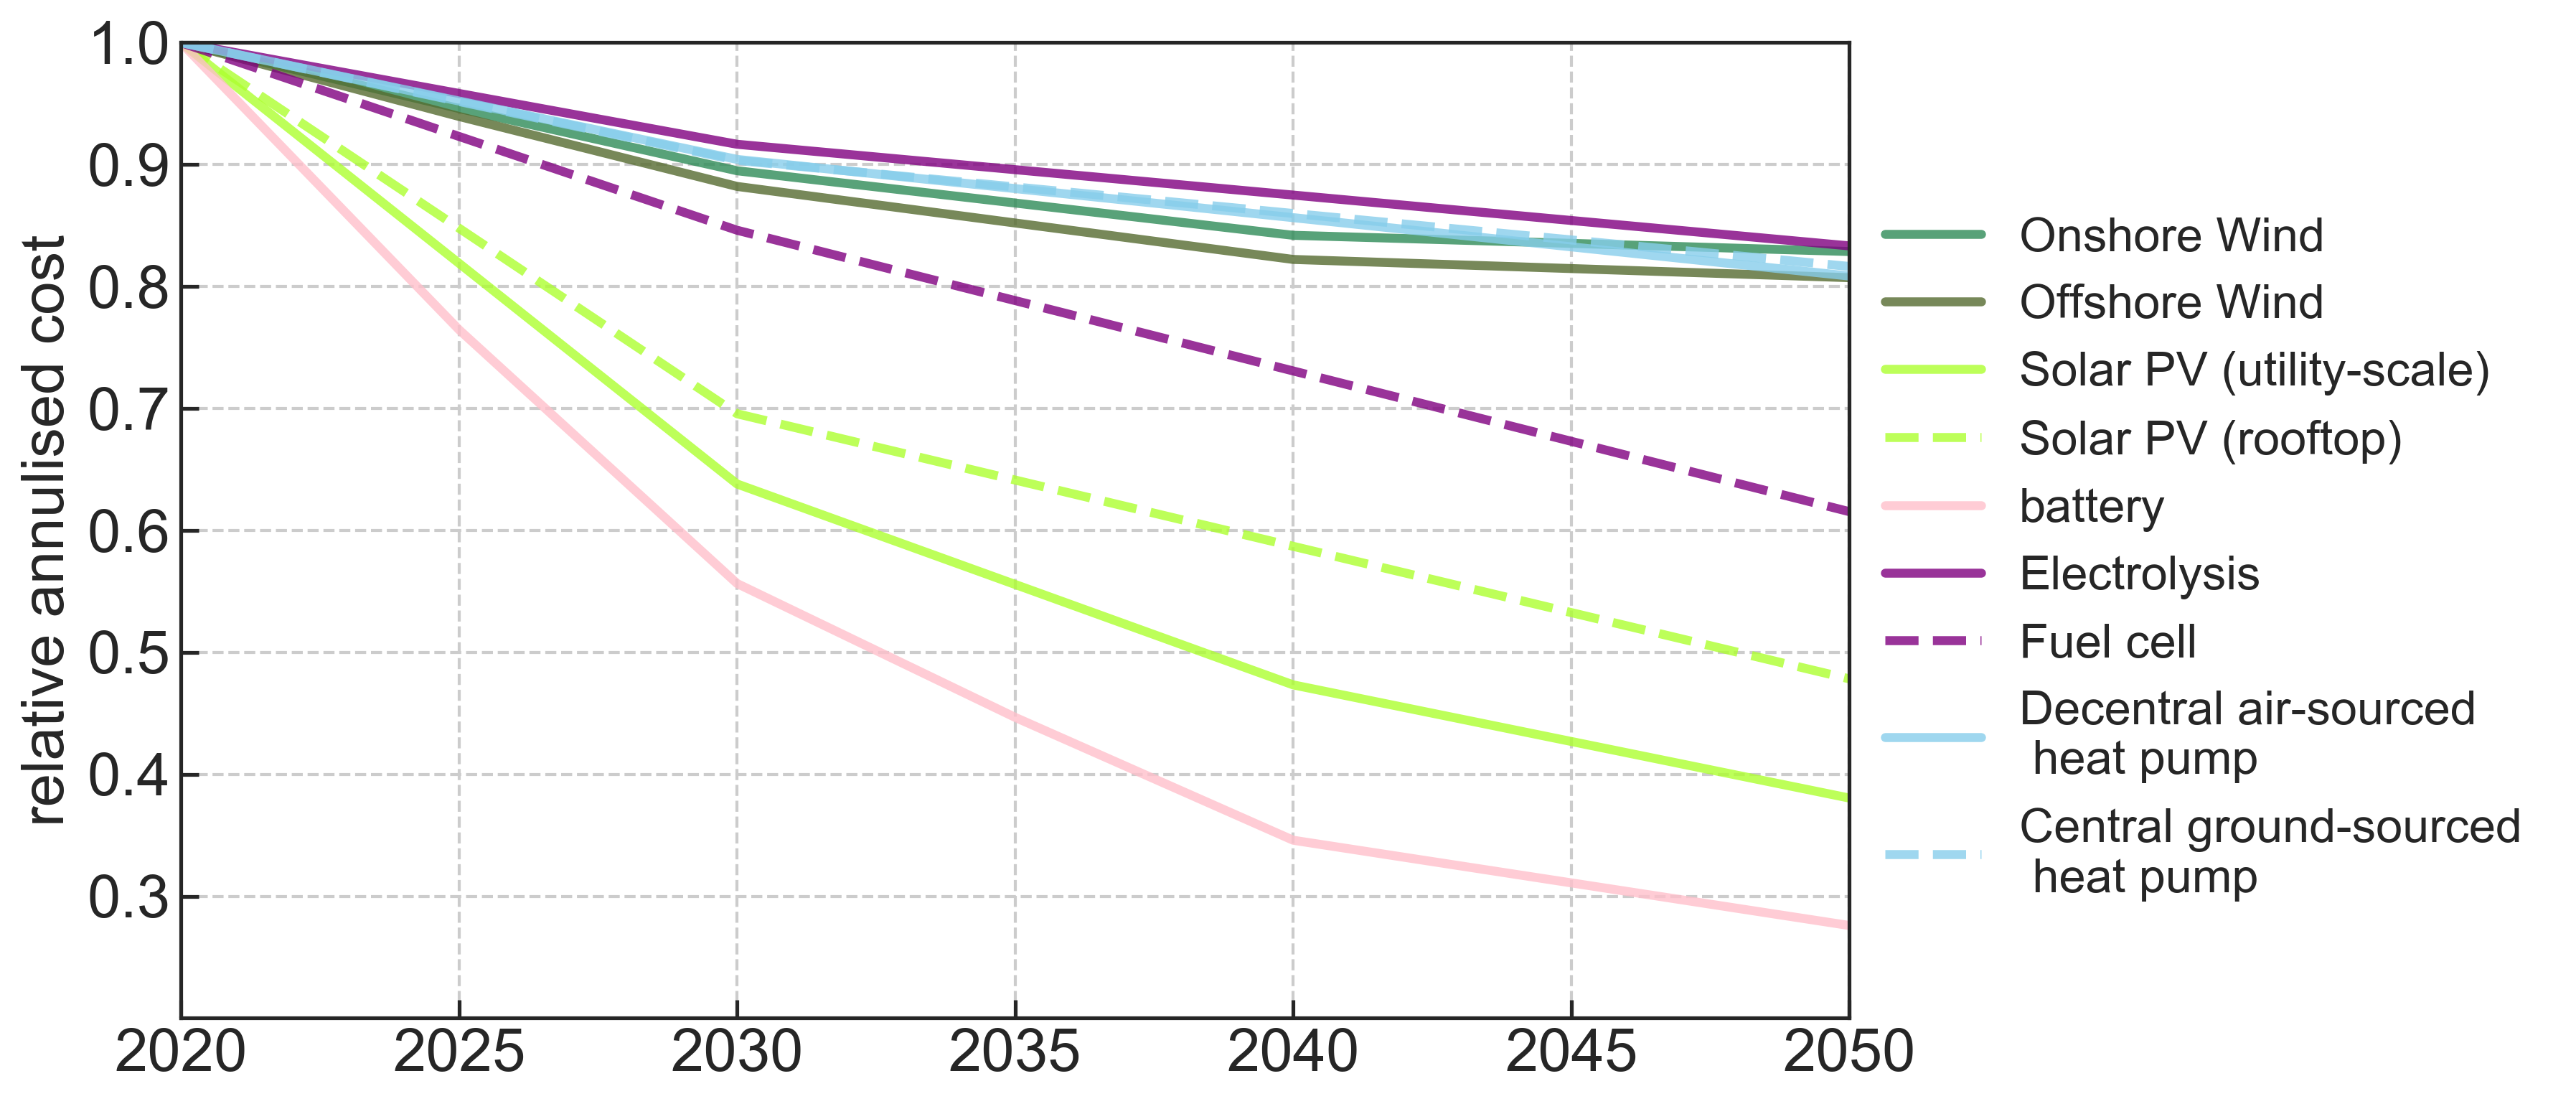
\includegraphics[width=12cm]{figures/cost_evolution.png}
\caption{Cost evolution assumed for the different technologies. } \label{fig_cost_evolution} 
\end{figure}


 
\section{References}
\bibliography{bib_transition}

\end{document}